\documentclass[1p]{elsarticle_modified}
%\bibliographystyle{elsarticle-num}

%\usepackage[colorlinks]{hyperref}
%\usepackage{abbrmath_seonhwa} %\Abb, \Ascr, \Acal ,\Abf, \Afrak
\usepackage{amsfonts}
\usepackage{amssymb}
\usepackage{amsmath}
\usepackage{amsthm}
\usepackage{scalefnt}
\usepackage{amsbsy}
\usepackage{kotex}
\usepackage{caption}
\usepackage{subfig}
\usepackage{color}
\usepackage{graphicx}
\usepackage{xcolor} %% white, black, red, green, blue, cyan, magenta, yellow
\usepackage{float}
\usepackage{setspace}
\usepackage{hyperref}

\usepackage{tikz}
\usetikzlibrary{arrows}

\usepackage{multirow}
\usepackage{array} % fixed length table
\usepackage{hhline}

%%%%%%%%%%%%%%%%%%%%%
\makeatletter
\renewcommand*\env@matrix[1][\arraystretch]{%
	\edef\arraystretch{#1}%
	\hskip -\arraycolsep
	\let\@ifnextchar\new@ifnextchar
	\array{*\c@MaxMatrixCols c}}
\makeatother %https://tex.stackexchange.com/questions/14071/how-can-i-increase-the-line-spacing-in-a-matrix
%%%%%%%%%%%%%%%

\usepackage[normalem]{ulem}

\newcommand{\msout}[1]{\ifmmode\text{\sout{\ensuremath{#1}}}\else\sout{#1}\fi}
%SOURCE: \msout is \stkout macro in https://tex.stackexchange.com/questions/20609/strikeout-in-math-mode

\newcommand{\cancel}[1]{
	\ifmmode
	{\color{red}\msout{#1}}
	\else
	{\color{red}\sout{#1}}
	\fi
}

\newcommand{\add}[1]{
	{\color{blue}\uwave{#1}}
}

\newcommand{\replace}[2]{
	\ifmmode
	{\color{red}\msout{#1}}{\color{blue}\uwave{#2}}
	\else
	{\color{red}\sout{#1}}{\color{blue}\uwave{#2}}
	\fi
}

\newcommand{\Sol}{\mathcal{S}} %segment
\newcommand{\D}{D} %diagram
\newcommand{\A}{\mathcal{A}} %arc


%%%%%%%%%%%%%%%%%%%%%%%%%%%%%5 test

\def\sl{\operatorname{\textup{SL}}(2,\Cbb)}
\def\psl{\operatorname{\textup{PSL}}(2,\Cbb)}
\def\quan{\mkern 1mu \triangleright \mkern 1mu}

\theoremstyle{definition}
\newtheorem{thm}{Theorem}[section]
\newtheorem{prop}[thm]{Proposition}
\newtheorem{lem}[thm]{Lemma}
\newtheorem{ques}[thm]{Question}
\newtheorem{cor}[thm]{Corollary}
\newtheorem{defn}[thm]{Definition}
\newtheorem{exam}[thm]{Example}
\newtheorem{rmk}[thm]{Remark}
\newtheorem{alg}[thm]{Algorithm}

\newcommand{\I}{\sqrt{-1}}
\begin{document}

%\begin{frontmatter}
%
%\title{Boundary parabolic representations of knots up to 8 crossings}
%
%%% Group authors per affiliation:
%\author{Yunhi Cho} 
%\address{Department of Mathematics, University of Seoul, Seoul, Korea}
%\ead{yhcho@uos.ac.kr}
%
%
%\author{Seonhwa Kim} %\fnref{s_kim}}
%\address{Center for Geometry and Physics, Institute for Basic Science, Pohang, 37673, Korea}
%\ead{ryeona17@ibs.re.kr}
%
%\author{Hyuk Kim}
%\address{Department of Mathematical Sciences, Seoul National University, Seoul 08826, Korea}
%\ead{hyukkim@snu.ac.kr}
%
%\author{Seokbeom Yoon}
%\address{Department of Mathematical Sciences, Seoul National University, Seoul, 08826,  Korea}
%\ead{sbyoon15@snu.ac.kr}
%
%\begin{abstract}
%We find all boundary parabolic representation of knots up to 8 crossings.
%
%\end{abstract}
%\begin{keyword}
%    \MSC[2010] 57M25 
%\end{keyword}
%
%\end{frontmatter}

%\linenumbers
%\tableofcontents
%
\newcommand\colored[1]{\textcolor{white}{\rule[-0.35ex]{0.8em}{1.4ex}}\kern-0.8em\color{red} #1}%
%\newcommand\colored[1]{\textcolor{white}{ #1}\kern-2.17ex	\textcolor{white}{ #1}\kern-1.81ex	\textcolor{white}{ #1}\kern-2.15ex\color{red}#1	}

{\Large $\underline{12a_{0979}~(K12a_{0979})}$}

\setlength{\tabcolsep}{10pt}
\renewcommand{\arraystretch}{1.6}
\vspace{1cm}\begin{tabular}{m{100pt}>{\centering\arraybackslash}m{274pt}}
\multirow{5}{120pt}{
	\centering
	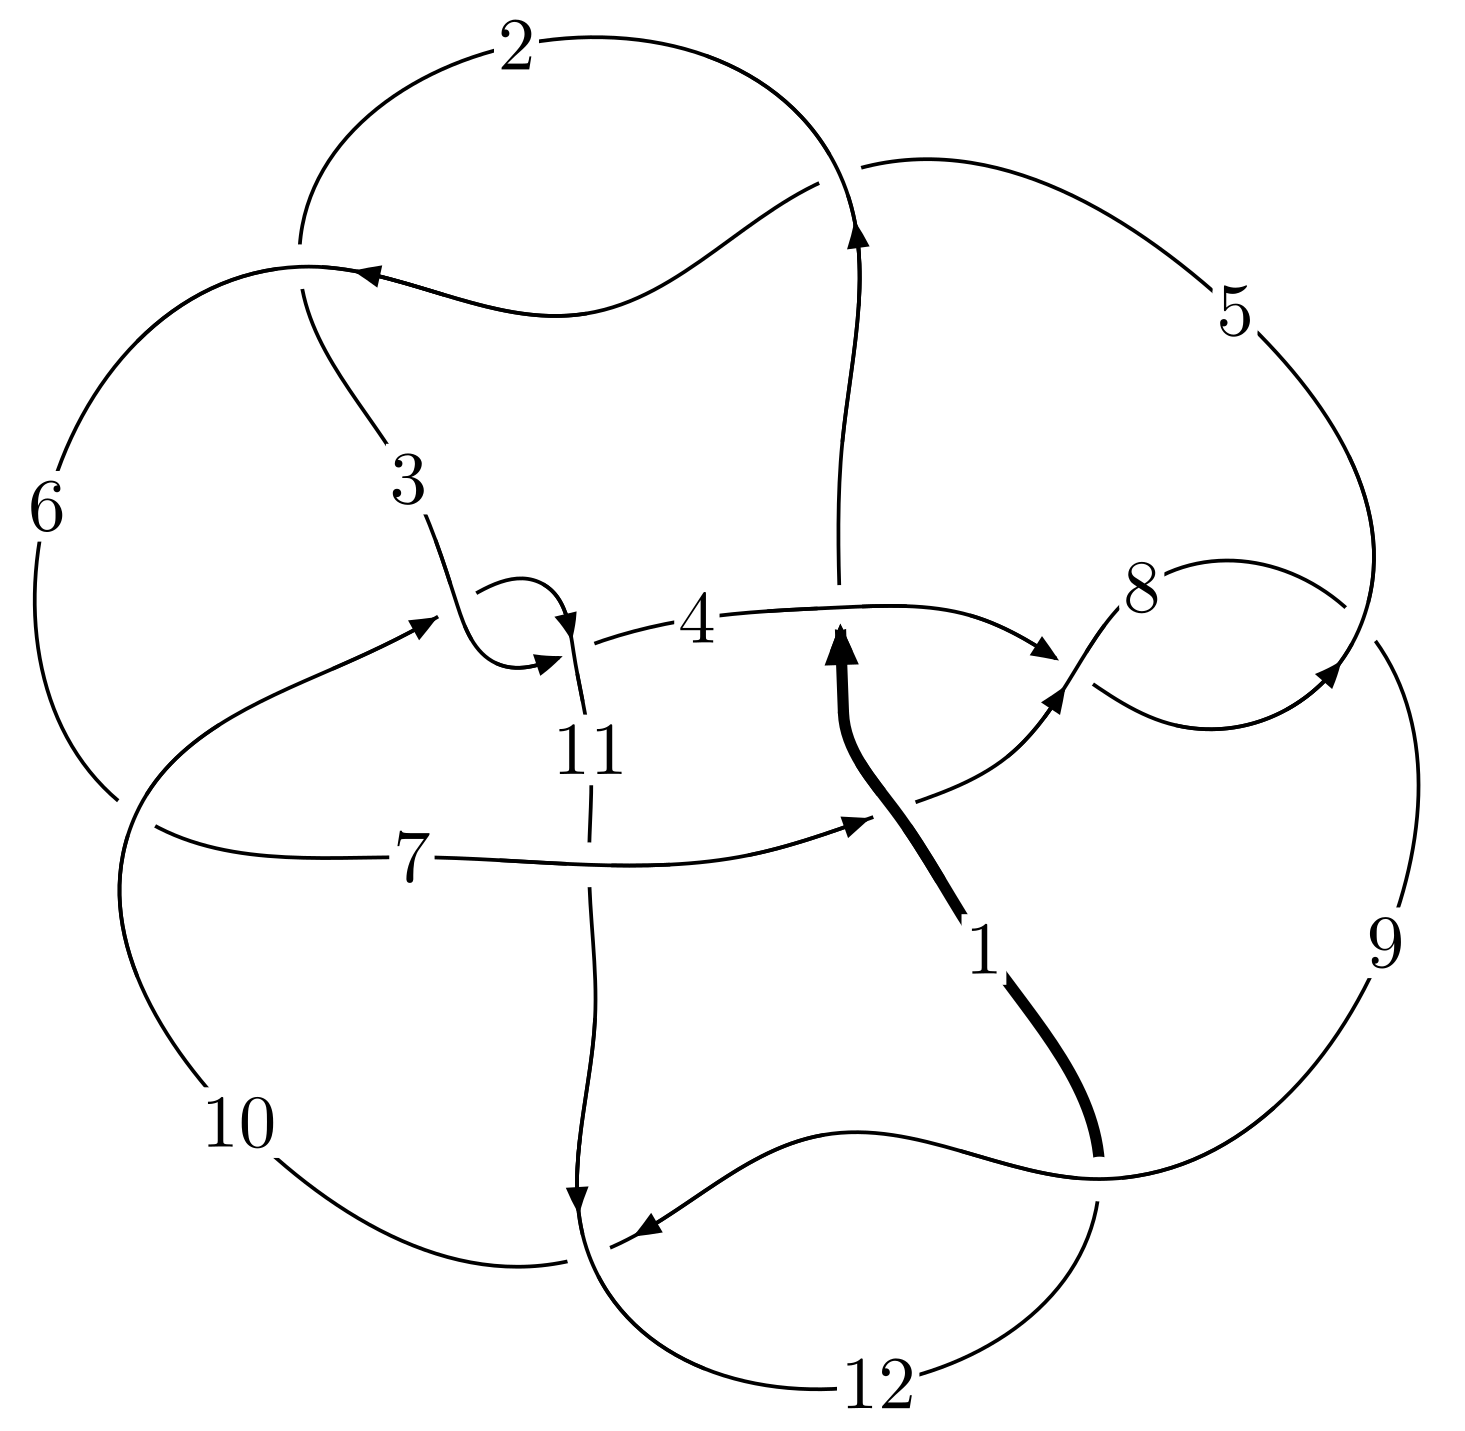
\includegraphics[width=112pt]{../../../GIT/diagram.site/Diagrams/png/1780_12a_0979.png}\\
\ \ \ A knot diagram\footnotemark}&
\allowdisplaybreaks
\textbf{Linearized knot diagam} \\
\cline{2-2}
 &
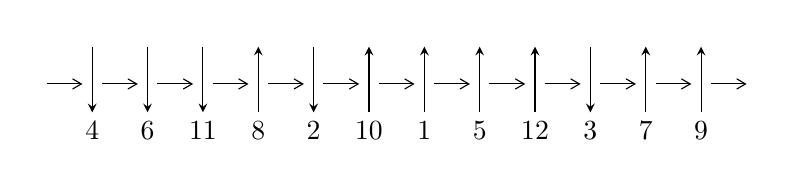
\begin{tikzpicture}[x=20pt, y=17pt]
	% nodes
	\node (C0) at (0, 0) {};
	\node (C1) at (1, 0) {};
	\node (C1U) at (1, +1) {};
	\node (C1D) at (1, -1) {4};

	\node (C2) at (2, 0) {};
	\node (C2U) at (2, +1) {};
	\node (C2D) at (2, -1) {6};

	\node (C3) at (3, 0) {};
	\node (C3U) at (3, +1) {};
	\node (C3D) at (3, -1) {11};

	\node (C4) at (4, 0) {};
	\node (C4U) at (4, +1) {};
	\node (C4D) at (4, -1) {8};

	\node (C5) at (5, 0) {};
	\node (C5U) at (5, +1) {};
	\node (C5D) at (5, -1) {2};

	\node (C6) at (6, 0) {};
	\node (C6U) at (6, +1) {};
	\node (C6D) at (6, -1) {10};

	\node (C7) at (7, 0) {};
	\node (C7U) at (7, +1) {};
	\node (C7D) at (7, -1) {1};

	\node (C8) at (8, 0) {};
	\node (C8U) at (8, +1) {};
	\node (C8D) at (8, -1) {5};

	\node (C9) at (9, 0) {};
	\node (C9U) at (9, +1) {};
	\node (C9D) at (9, -1) {12};

	\node (C10) at (10, 0) {};
	\node (C10U) at (10, +1) {};
	\node (C10D) at (10, -1) {3};

	\node (C11) at (11, 0) {};
	\node (C11U) at (11, +1) {};
	\node (C11D) at (11, -1) {7};

	\node (C12) at (12, 0) {};
	\node (C12U) at (12, +1) {};
	\node (C12D) at (12, -1) {9};
	\node (C13) at (13, 0) {};

	% arrows
	\draw[->,>={angle 60}]
	(C0) edge (C1) (C1) edge (C2) (C2) edge (C3) (C3) edge (C4) (C4) edge (C5) (C5) edge (C6) (C6) edge (C7) (C7) edge (C8) (C8) edge (C9) (C9) edge (C10) (C10) edge (C11) (C11) edge (C12) (C12) edge (C13) ;	\draw[->,>=stealth]
	(C1U) edge (C1D) (C2U) edge (C2D) (C3U) edge (C3D) (C4D) edge (C4U) (C5U) edge (C5D) (C6D) edge (C6U) (C7D) edge (C7U) (C8D) edge (C8U) (C9D) edge (C9U) (C10U) edge (C10D) (C11D) edge (C11U) (C12D) edge (C12U) ;
	\end{tikzpicture} \\
\hhline{~~} \\& 
\textbf{Solving Sequence} \\ \cline{2-2} 
 &
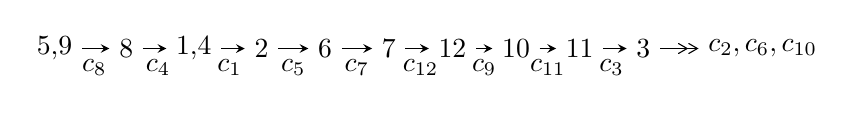
\begin{tikzpicture}[x=23pt, y=7pt]
	% node
	\node (A0) at (-1/8, 0) {5,9};
	\node (A1) at (1, 0) {8};
	\node (A2) at (33/16, 0) {1,4};
	\node (A3) at (25/8, 0) {2};
	\node (A4) at (33/8, 0) {6};
	\node (A5) at (41/8, 0) {7};
	\node (A6) at (49/8, 0) {12};
	\node (A7) at (57/8, 0) {10};
	\node (A8) at (65/8, 0) {11};
	\node (A9) at (73/8, 0) {3};
	\node (C1) at (1/2, -1) {$c_{8}$};
	\node (C2) at (3/2, -1) {$c_{4}$};
	\node (C3) at (21/8, -1) {$c_{1}$};
	\node (C4) at (29/8, -1) {$c_{5}$};
	\node (C5) at (37/8, -1) {$c_{7}$};
	\node (C6) at (45/8, -1) {$c_{12}$};
	\node (C7) at (53/8, -1) {$c_{9}$};
	\node (C8) at (61/8, -1) {$c_{11}$};
	\node (C9) at (69/8, -1) {$c_{3}$};
	\node (A10) at (11, 0) {$c_{2},c_{6},c_{10}$};

	% edge
	\draw[->,>=stealth]	
	(A0) edge (A1) (A1) edge (A2) (A2) edge (A3) (A3) edge (A4) (A4) edge (A5) (A5) edge (A6) (A6) edge (A7) (A7) edge (A8) (A8) edge (A9) ;
	\draw[->>,>={angle 60}]	
	(A9) edge (A10);
\end{tikzpicture} \\ 

\end{tabular} \\

\footnotetext{
The image of knot diagram is generated by the software ``\textbf{Draw programme}" developed by Andrew Bartholomew(\url{http://www.layer8.co.uk/maths/draw/index.htm\#Running-draw}), where we modified some parts for our purpose(\url{https://github.com/CATsTAILs/LinksPainter}).
}\phantom \\ \newline 
\centering \textbf{Ideals for irreducible components\footnotemark of $X_{\text{par}}$} 
 
\begin{align*}
I^u_{1}&=\langle 
1.28281\times10^{609} u^{152}+5.70333\times10^{609} u^{151}+\cdots+1.62531\times10^{610} b+4.43748\times10^{612},\\
\phantom{I^u_{1}}&\phantom{= \langle  }9.86064\times10^{612} u^{152}+3.28103\times10^{613} u^{151}+\cdots+4.53298\times10^{613} a+4.56455\times10^{616},\\
\phantom{I^u_{1}}&\phantom{= \langle  }u^{153}+3 u^{152}+\cdots-5927 u-2789\rangle \\
I^u_{2}&=\langle 
-4.96325\times10^{19} u^{36}-1.68009\times10^{20} u^{35}+\cdots+5.82980\times10^{17} b+9.18197\times10^{19},\\
\phantom{I^u_{2}}&\phantom{= \langle  }2.83565\times10^{19} u^{36}+9.47056\times10^{19} u^{35}+\cdots+5.82980\times10^{17} a-7.12118\times10^{19},\;u^{37}+4 u^{36}+\cdots-8 u-1\rangle \\
I^u_{3}&=\langle 
b,\;a- u-1,\;u^3+u^2-1\rangle \\
I^u_{4}&=\langle 
b,\;a-1,\;u-1\rangle \\
\\
\end{align*}
\raggedright * 4 irreducible components of $\dim_{\mathbb{C}}=0$, with total 194 representations.\\
\footnotetext{All coefficients of polynomials are rational numbers. But the coefficients are sometimes approximated in decimal forms when there is not enough margin.}
\newpage
\renewcommand{\arraystretch}{1}
\centering \section*{I. $I^u_{1}= \langle 1.28\times10^{609} u^{152}+5.70\times10^{609} u^{151}+\cdots+1.63\times10^{610} b+4.44\times10^{612},\;9.86\times10^{612} u^{152}+3.28\times10^{613} u^{151}+\cdots+4.53\times10^{613} a+4.56\times10^{616},\;u^{153}+3 u^{152}+\cdots-5927 u-2789 \rangle$}
\flushleft \textbf{(i) Arc colorings}\\
\begin{tabular}{m{7pt} m{180pt} m{7pt} m{180pt} }
\flushright $a_{5}=$&$\begin{pmatrix}0\\u\end{pmatrix}$ \\
\flushright $a_{9}=$&$\begin{pmatrix}1\\0\end{pmatrix}$ \\
\flushright $a_{8}=$&$\begin{pmatrix}1\\u^2\end{pmatrix}$ \\
\flushright $a_{1}=$&$\begin{pmatrix}-0.217531 u^{152}-0.723812 u^{151}+\cdots-2983.07 u-1006.96\\-0.0789275 u^{152}-0.350907 u^{151}+\cdots-1126.14 u-273.024\end{pmatrix}$ \\
\flushright $a_{4}=$&$\begin{pmatrix}- u\\- u^3+u\end{pmatrix}$ \\
\flushright $a_{2}=$&$\begin{pmatrix}-0.104395 u^{152}-0.284179 u^{151}+\cdots-1526.20 u-473.627\\-0.0380832 u^{152}-0.244056 u^{151}+\cdots-1673.44 u-526.835\end{pmatrix}$ \\
\flushright $a_{6}=$&$\begin{pmatrix}1.88754 u^{152}+7.27310 u^{151}+\cdots+19454.7 u+5679.34\\-0.431277 u^{152}-1.74643 u^{151}+\cdots-5970.32 u-1834.41\end{pmatrix}$ \\
\flushright $a_{7}=$&$\begin{pmatrix}2.38322 u^{152}+9.22443 u^{151}+\cdots+26525.4 u+8607.01\\-0.204594 u^{152}-1.05976 u^{151}+\cdots-5337.10 u-1970.55\end{pmatrix}$ \\
\flushright $a_{12}=$&$\begin{pmatrix}-0.138603 u^{152}-0.372904 u^{151}+\cdots-1856.93 u-733.940\\-0.0789275 u^{152}-0.350907 u^{151}+\cdots-1126.14 u-273.024\end{pmatrix}$ \\
\flushright $a_{10}=$&$\begin{pmatrix}-0.501318 u^{152}-2.22897 u^{151}+\cdots-9009.17 u-2879.10\\0.247246 u^{152}+1.06495 u^{151}+\cdots+2246.96 u+849.901\end{pmatrix}$ \\
\flushright $a_{11}=$&$\begin{pmatrix}6.22371 u^{152}+24.5377 u^{151}+\cdots+57732.8 u+18511.5\\-0.738844 u^{152}-3.16251 u^{151}+\cdots-6523.56 u-2353.66\end{pmatrix}$ \\
\flushright $a_{3}=$&$\begin{pmatrix}-6.52573 u^{152}-26.1053 u^{151}+\cdots-59538.9 u-18890.0\\0.571964 u^{152}+2.31321 u^{151}+\cdots+3012.92 u+903.759\end{pmatrix}$\\&\end{tabular}
\flushleft \textbf{(ii) Obstruction class $= -1$}\\~\\
\flushleft \textbf{(iii) Cusp Shapes $= 5.81594 u^{152}+24.7068 u^{151}+\cdots+47717.7 u+16629.8$}\\~\\
\newpage\renewcommand{\arraystretch}{1}
\flushleft \textbf{(iv) u-Polynomials at the component}\newline \\
\begin{tabular}{m{50pt}|m{274pt}}
Crossings & \hspace{64pt}u-Polynomials at each crossing \\
\hline $$\begin{aligned}c_{1}\end{aligned}$$&$\begin{aligned}
&u^{153}-12 u^{152}+\cdots-56332 u+7874
\end{aligned}$\\
\hline $$\begin{aligned}c_{2},c_{5}\end{aligned}$$&$\begin{aligned}
&u^{153}+9 u^{152}+\cdots-508434 u-176401
\end{aligned}$\\
\hline $$\begin{aligned}c_{3},c_{10}\end{aligned}$$&$\begin{aligned}
&u^{153}-3 u^{152}+\cdots+28708 u-3617
\end{aligned}$\\
\hline $$\begin{aligned}c_{4},c_{8}\end{aligned}$$&$\begin{aligned}
&u^{153}+3 u^{152}+\cdots-5927 u-2789
\end{aligned}$\\
\hline $$\begin{aligned}c_{6}\end{aligned}$$&$\begin{aligned}
&u^{153}-7 u^{152}+\cdots-4234131617 u-264250321
\end{aligned}$\\
\hline $$\begin{aligned}c_{7}\end{aligned}$$&$\begin{aligned}
&u^{153}+3 u^{152}+\cdots+1096 u-428
\end{aligned}$\\
\hline $$\begin{aligned}c_{9},c_{12}\end{aligned}$$&$\begin{aligned}
&u^{153}+10 u^{152}+\cdots+6400 u-2432
\end{aligned}$\\
\hline $$\begin{aligned}c_{11}\end{aligned}$$&$\begin{aligned}
&u^{153}+15 u^{152}+\cdots+331308 u-100816
\end{aligned}$\\
\hline
\end{tabular}\\~\\
\newpage\renewcommand{\arraystretch}{1}
\flushleft \textbf{(v) Riley Polynomials at the component}\newline \\
\begin{tabular}{m{50pt}|m{274pt}}
Crossings & \hspace{64pt}Riley Polynomials at each crossing \\
\hline $$\begin{aligned}c_{1}\end{aligned}$$&$\begin{aligned}
&y^{153}+20 y^{152}+\cdots+105095636 y-61999876
\end{aligned}$\\
\hline $$\begin{aligned}c_{2},c_{5}\end{aligned}$$&$\begin{aligned}
&y^{153}-193 y^{152}+\cdots+755521653094 y-31117312801
\end{aligned}$\\
\hline $$\begin{aligned}c_{3},c_{10}\end{aligned}$$&$\begin{aligned}
&y^{153}-105 y^{152}+\cdots+1173688910 y-13082689
\end{aligned}$\\
\hline $$\begin{aligned}c_{4},c_{8}\end{aligned}$$&$\begin{aligned}
&y^{153}-75 y^{152}+\cdots+149372347 y-7778521
\end{aligned}$\\
\hline $$\begin{aligned}c_{6}\end{aligned}$$&$\begin{aligned}
&y^{153}+77 y^{152}+\cdots+1847642535511061561 y-69828232148603041
\end{aligned}$\\
\hline $$\begin{aligned}c_{7}\end{aligned}$$&$\begin{aligned}
&y^{153}-75 y^{152}+\cdots+8936032 y-183184
\end{aligned}$\\
\hline $$\begin{aligned}c_{9},c_{12}\end{aligned}$$&$\begin{aligned}
&y^{153}+118 y^{152}+\cdots+647831552 y-5914624
\end{aligned}$\\
\hline $$\begin{aligned}c_{11}\end{aligned}$$&$\begin{aligned}
&y^{153}-35 y^{152}+\cdots+290394396848 y-10163865856
\end{aligned}$\\
\hline
\end{tabular}\\~\\
\newpage\flushleft \textbf{(vi) Complex Volumes and Cusp Shapes}
$$\begin{array}{c|c|c}  
\text{Solutions to }I^u_{1}& \I (\text{vol} + \sqrt{-1}CS) & \text{Cusp shape}\\
 \hline 
\begin{aligned}
u &= \phantom{-}0.997781\phantom{ +0.000000I} \\
a &= \phantom{-}8.75197\phantom{ +0.000000I} \\
b &= \phantom{-}0.0647899\phantom{ +0.000000I}\end{aligned}
 & -0.00219509\phantom{ +0.000000I} & \phantom{-0.000000 } 0 \\ \hline\begin{aligned}
u &= -0.341614 + 0.931233 I \\
a &= -0.370406 + 0.406647 I \\
b &= -0.185584 - 1.072250 I\end{aligned}
 & -3.61191 + 2.52822 I & \phantom{-0.000000 } 0 \\ \hline\begin{aligned}
u &= -0.341614 - 0.931233 I \\
a &= -0.370406 - 0.406647 I \\
b &= -0.185584 + 1.072250 I\end{aligned}
 & -3.61191 - 2.52822 I & \phantom{-0.000000 } 0 \\ \hline\begin{aligned}
u &= -0.072377 + 0.983268 I \\
a &= -0.318149 + 0.469174 I \\
b &= -0.300070 - 1.335890 I\end{aligned}
 & -5.26544 + 7.42458 I & \phantom{-0.000000 } 0 \\ \hline\begin{aligned}
u &= -0.072377 - 0.983268 I \\
a &= -0.318149 - 0.469174 I \\
b &= -0.300070 + 1.335890 I\end{aligned}
 & -5.26544 - 7.42458 I & \phantom{-0.000000 } 0 \\ \hline\begin{aligned}
u &= \phantom{-}0.864802 + 0.538644 I \\
a &= \phantom{-}1.02477 - 1.09021 I \\
b &= \phantom{-}0.244675 + 0.892365 I\end{aligned}
 & -0.76159 + 1.35256 I & \phantom{-0.000000 } 0 \\ \hline\begin{aligned}
u &= \phantom{-}0.864802 - 0.538644 I \\
a &= \phantom{-}1.02477 + 1.09021 I \\
b &= \phantom{-}0.244675 - 0.892365 I\end{aligned}
 & -0.76159 - 1.35256 I & \phantom{-0.000000 } 0 \\ \hline\begin{aligned}
u &= -0.827905 + 0.595560 I \\
a &= \phantom{-}1.304940 - 0.197851 I \\
b &= \phantom{-}0.12160 - 1.47494 I\end{aligned}
 & -8.89019 - 3.19697 I & \phantom{-0.000000 } 0 \\ \hline\begin{aligned}
u &= -0.827905 - 0.595560 I \\
a &= \phantom{-}1.304940 + 0.197851 I \\
b &= \phantom{-}0.12160 + 1.47494 I\end{aligned}
 & -8.89019 + 3.19697 I & \phantom{-0.000000 } 0 \\ \hline\begin{aligned}
u &= -0.025248 + 0.969006 I \\
a &= -0.299791 - 0.487821 I \\
b &= \phantom{-}0.906922 + 0.100199 I\end{aligned}
 & -2.14800 - 1.50633 I & \phantom{-0.000000 } 0\\
 \hline 
 \end{array}$$\newpage$$\begin{array}{c|c|c}  
\text{Solutions to }I^u_{1}& \I (\text{vol} + \sqrt{-1}CS) & \text{Cusp shape}\\
 \hline 
\begin{aligned}
u &= -0.025248 - 0.969006 I \\
a &= -0.299791 + 0.487821 I \\
b &= \phantom{-}0.906922 - 0.100199 I\end{aligned}
 & -2.14800 + 1.50633 I & \phantom{-0.000000 } 0 \\ \hline\begin{aligned}
u &= \phantom{-}0.989734 + 0.318008 I \\
a &= \phantom{-}0.22701 + 1.42246 I \\
b &= -0.70870 + 2.08315 I\end{aligned}
 & -7.32709 + 4.58957 I & \phantom{-0.000000 } 0 \\ \hline\begin{aligned}
u &= \phantom{-}0.989734 - 0.318008 I \\
a &= \phantom{-}0.22701 - 1.42246 I \\
b &= -0.70870 - 2.08315 I\end{aligned}
 & -7.32709 - 4.58957 I & \phantom{-0.000000 } 0 \\ \hline\begin{aligned}
u &= -0.902372 + 0.538652 I \\
a &= -1.090840 - 0.663576 I \\
b &= -0.13790 + 1.55018 I\end{aligned}
 & -9.00785 - 0.43770 I & \phantom{-0.000000 } 0 \\ \hline\begin{aligned}
u &= -0.902372 - 0.538652 I \\
a &= -1.090840 + 0.663576 I \\
b &= -0.13790 - 1.55018 I\end{aligned}
 & -9.00785 + 0.43770 I & \phantom{-0.000000 } 0 \\ \hline\begin{aligned}
u &= -0.862240 + 0.392691 I \\
a &= -0.29420 - 1.42358 I \\
b &= -0.161096 + 1.356630 I\end{aligned}
 & -9.38534 - 9.47300 I & \phantom{-0.000000 } 0 \\ \hline\begin{aligned}
u &= -0.862240 - 0.392691 I \\
a &= -0.29420 + 1.42358 I \\
b &= -0.161096 - 1.356630 I\end{aligned}
 & -9.38534 + 9.47300 I & \phantom{-0.000000 } 0 \\ \hline\begin{aligned}
u &= \phantom{-}0.832026 + 0.426042 I \\
a &= -0.293205 + 0.324712 I \\
b &= -0.48148 + 1.50098 I\end{aligned}
 & -9.63438 - 5.81743 I & \phantom{-0.000000 } 0 \\ \hline\begin{aligned}
u &= \phantom{-}0.832026 - 0.426042 I \\
a &= -0.293205 - 0.324712 I \\
b &= -0.48148 - 1.50098 I\end{aligned}
 & -9.63438 + 5.81743 I & \phantom{-0.000000 } 0 \\ \hline\begin{aligned}
u &= -0.119562 + 0.924520 I \\
a &= \phantom{-}0.096611 - 0.517704 I \\
b &= \phantom{-}0.349672 + 1.234820 I\end{aligned}
 & -2.18119 + 3.63455 I & \phantom{-0.000000 } 0\\
 \hline 
 \end{array}$$\newpage$$\begin{array}{c|c|c}  
\text{Solutions to }I^u_{1}& \I (\text{vol} + \sqrt{-1}CS) & \text{Cusp shape}\\
 \hline 
\begin{aligned}
u &= -0.119562 - 0.924520 I \\
a &= \phantom{-}0.096611 + 0.517704 I \\
b &= \phantom{-}0.349672 - 1.234820 I\end{aligned}
 & -2.18119 - 3.63455 I & \phantom{-0.000000 } 0 \\ \hline\begin{aligned}
u &= -0.826872 + 0.428150 I \\
a &= \phantom{-}0.252811 + 0.823012 I \\
b &= \phantom{-}0.093204 - 1.393210 I\end{aligned}
 & -5.75444 - 4.67554 I & \phantom{-0.000000 } 0 \\ \hline\begin{aligned}
u &= -0.826872 - 0.428150 I \\
a &= \phantom{-}0.252811 - 0.823012 I \\
b &= \phantom{-}0.093204 + 1.393210 I\end{aligned}
 & -5.75444 + 4.67554 I & \phantom{-0.000000 } 0 \\ \hline\begin{aligned}
u &= -0.726161 + 0.582004 I \\
a &= -0.737072 + 0.151735 I \\
b &= -0.00296 + 1.53384 I\end{aligned}
 & -9.17623 - 1.44438 I & \phantom{-0.000000 } 0 \\ \hline\begin{aligned}
u &= -0.726161 - 0.582004 I \\
a &= -0.737072 - 0.151735 I \\
b &= -0.00296 - 1.53384 I\end{aligned}
 & -9.17623 + 1.44438 I & \phantom{-0.000000 } 0 \\ \hline\begin{aligned}
u &= \phantom{-}0.882528 + 0.290522 I \\
a &= \phantom{-}1.85197 - 1.11541 I \\
b &= \phantom{-}0.383224 - 0.566013 I\end{aligned}
 & \phantom{-}1.56920 + 3.18136 I & \phantom{-0.000000 } 0 \\ \hline\begin{aligned}
u &= \phantom{-}0.882528 - 0.290522 I \\
a &= \phantom{-}1.85197 + 1.11541 I \\
b &= \phantom{-}0.383224 + 0.566013 I\end{aligned}
 & \phantom{-}1.56920 - 3.18136 I & \phantom{-0.000000 } 0 \\ \hline\begin{aligned}
u &= -0.899606 + 0.585036 I \\
a &= -0.394547 + 0.708643 I \\
b &= \phantom{-}0.043813 + 0.711490 I\end{aligned}
 & -0.935418 + 0.215869 I & \phantom{-0.000000 } 0 \\ \hline\begin{aligned}
u &= -0.899606 - 0.585036 I \\
a &= -0.394547 - 0.708643 I \\
b &= \phantom{-}0.043813 - 0.711490 I\end{aligned}
 & -0.935418 - 0.215869 I & \phantom{-0.000000 } 0 \\ \hline\begin{aligned}
u &= \phantom{-}0.861926 + 0.334675 I \\
a &= \phantom{-}2.55635 + 0.76486 I \\
b &= \phantom{-}0.56596 + 1.48467 I\end{aligned}
 & -5.08208 + 4.36622 I & \phantom{-0.000000 } 0\\
 \hline 
 \end{array}$$\newpage$$\begin{array}{c|c|c}  
\text{Solutions to }I^u_{1}& \I (\text{vol} + \sqrt{-1}CS) & \text{Cusp shape}\\
 \hline 
\begin{aligned}
u &= \phantom{-}0.861926 - 0.334675 I \\
a &= \phantom{-}2.55635 - 0.76486 I \\
b &= \phantom{-}0.56596 - 1.48467 I\end{aligned}
 & -5.08208 - 4.36622 I & \phantom{-0.000000 } 0 \\ \hline\begin{aligned}
u &= \phantom{-}0.088621 + 0.920266 I \\
a &= \phantom{-}0.031760 + 0.517902 I \\
b &= -0.981938 + 0.073899 I\end{aligned}
 & -6.10163 - 8.06042 I & \phantom{-0.000000 } 0 \\ \hline\begin{aligned}
u &= \phantom{-}0.088621 - 0.920266 I \\
a &= \phantom{-}0.031760 - 0.517902 I \\
b &= -0.981938 - 0.073899 I\end{aligned}
 & -6.10163 + 8.06042 I & \phantom{-0.000000 } 0 \\ \hline\begin{aligned}
u &= \phantom{-}0.824328 + 0.409646 I \\
a &= -2.59398 - 0.67280 I \\
b &= -0.69516 - 1.29223 I\end{aligned}
 & -9.66879 + 9.36370 I & \phantom{-0.000000 } 0 \\ \hline\begin{aligned}
u &= \phantom{-}0.824328 - 0.409646 I \\
a &= -2.59398 + 0.67280 I \\
b &= -0.69516 + 1.29223 I\end{aligned}
 & -9.66879 - 9.36370 I & \phantom{-0.000000 } 0 \\ \hline\begin{aligned}
u &= -0.800529 + 0.438940 I \\
a &= -2.50618 + 0.30716 I \\
b &= \phantom{-}0.081374 + 1.141410 I\end{aligned}
 & -5.83015 + 1.00845 I & \phantom{-0.000000 } 0 \\ \hline\begin{aligned}
u &= -0.800529 - 0.438940 I \\
a &= -2.50618 - 0.30716 I \\
b &= \phantom{-}0.081374 - 1.141410 I\end{aligned}
 & -5.83015 - 1.00845 I & \phantom{-0.000000 } 0 \\ \hline\begin{aligned}
u &= \phantom{-}1.045210 + 0.312312 I \\
a &= -1.042300 + 0.955080 I \\
b &= -0.333642 + 0.446226 I\end{aligned}
 & \phantom{-}2.12407 - 0.35100 I & \phantom{-0.000000 } 0 \\ \hline\begin{aligned}
u &= \phantom{-}1.045210 - 0.312312 I \\
a &= -1.042300 - 0.955080 I \\
b &= -0.333642 - 0.446226 I\end{aligned}
 & \phantom{-}2.12407 + 0.35100 I & \phantom{-0.000000 } 0 \\ \hline\begin{aligned}
u &= -0.247276 + 0.864800 I \\
a &= \phantom{-}0.349804 - 0.025716 I \\
b &= \phantom{-}0.427405 + 1.068930 I\end{aligned}
 & -5.34348 + 4.86562 I & \phantom{-0.000000 } 0\\
 \hline 
 \end{array}$$\newpage$$\begin{array}{c|c|c}  
\text{Solutions to }I^u_{1}& \I (\text{vol} + \sqrt{-1}CS) & \text{Cusp shape}\\
 \hline 
\begin{aligned}
u &= -0.247276 - 0.864800 I \\
a &= \phantom{-}0.349804 + 0.025716 I \\
b &= \phantom{-}0.427405 - 1.068930 I\end{aligned}
 & -5.34348 - 4.86562 I & \phantom{-0.000000 } 0 \\ \hline\begin{aligned}
u &= -0.809279 + 0.390526 I \\
a &= \phantom{-}3.04826 - 0.42221 I \\
b &= -0.138789 - 1.089010 I\end{aligned}
 & -9.56347 + 6.10996 I & \phantom{-0.000000 } 0 \\ \hline\begin{aligned}
u &= -0.809279 - 0.390526 I \\
a &= \phantom{-}3.04826 + 0.42221 I \\
b &= -0.138789 + 1.089010 I\end{aligned}
 & -9.56347 - 6.10996 I & \phantom{-0.000000 } 0 \\ \hline\begin{aligned}
u &= \phantom{-}0.826940 + 0.333273 I \\
a &= -0.405508 + 0.051029 I \\
b &= \phantom{-}0.27071 - 1.58027 I\end{aligned}
 & -5.19468 - 1.39926 I & \phantom{-0.000000 } 0 \\ \hline\begin{aligned}
u &= \phantom{-}0.826940 - 0.333273 I \\
a &= -0.405508 - 0.051029 I \\
b &= \phantom{-}0.27071 + 1.58027 I\end{aligned}
 & -5.19468 + 1.39926 I & \phantom{-0.000000 } 0 \\ \hline\begin{aligned}
u &= \phantom{-}1.098250 + 0.159299 I \\
a &= -0.807502 + 0.315922 I \\
b &= -0.252210 + 0.472759 I\end{aligned}
 & \phantom{-}2.04815 + 0.14892 I & \phantom{-0.000000 } 0 \\ \hline\begin{aligned}
u &= \phantom{-}1.098250 - 0.159299 I \\
a &= -0.807502 - 0.315922 I \\
b &= -0.252210 - 0.472759 I\end{aligned}
 & \phantom{-}2.04815 - 0.14892 I & \phantom{-0.000000 } 0 \\ \hline\begin{aligned}
u &= \phantom{-}0.882448 + 0.078541 I \\
a &= -2.64840 + 3.64459 I \\
b &= -0.00259 - 1.43722 I\end{aligned}
 & -5.21371 + 0.20813 I & \phantom{-0.000000 } 0 \\ \hline\begin{aligned}
u &= \phantom{-}0.882448 - 0.078541 I \\
a &= -2.64840 - 3.64459 I \\
b &= -0.00259 + 1.43722 I\end{aligned}
 & -5.21371 - 0.20813 I & \phantom{-0.000000 } 0 \\ \hline\begin{aligned}
u &= \phantom{-}1.040800 + 0.455931 I \\
a &= \phantom{-}2.37266 + 0.10421 I \\
b &= \phantom{-}0.294268 + 1.152880 I\end{aligned}
 & -0.60098 + 5.99532 I & \phantom{-0.000000 } 0\\
 \hline 
 \end{array}$$\newpage$$\begin{array}{c|c|c}  
\text{Solutions to }I^u_{1}& \I (\text{vol} + \sqrt{-1}CS) & \text{Cusp shape}\\
 \hline 
\begin{aligned}
u &= \phantom{-}1.040800 - 0.455931 I \\
a &= \phantom{-}2.37266 - 0.10421 I \\
b &= \phantom{-}0.294268 - 1.152880 I\end{aligned}
 & -0.60098 - 5.99532 I & \phantom{-0.000000 } 0 \\ \hline\begin{aligned}
u &= \phantom{-}0.855047\phantom{ +0.000000I} \\
a &= \phantom{-}2.44653\phantom{ +0.000000I} \\
b &= \phantom{-}0.623171\phantom{ +0.000000I}\end{aligned}
 & \phantom{-}0.683985\phantom{ +0.000000I} & \phantom{-0.000000 } 0 \\ \hline\begin{aligned}
u &= -1.052750 + 0.475909 I \\
a &= \phantom{-}1.17176 + 0.80525 I \\
b &= \phantom{-}0.947447 + 0.572850 I\end{aligned}
 & -0.93849 - 4.41930 I & \phantom{-0.000000 } 0 \\ \hline\begin{aligned}
u &= -1.052750 - 0.475909 I \\
a &= \phantom{-}1.17176 - 0.80525 I \\
b &= \phantom{-}0.947447 - 0.572850 I\end{aligned}
 & -0.93849 + 4.41930 I & \phantom{-0.000000 } 0 \\ \hline\begin{aligned}
u &= -0.829950 + 0.155484 I \\
a &= -1.56712 - 0.63356 I \\
b &= -1.007240 - 0.465181 I\end{aligned}
 & -1.68823 - 1.09179 I & \phantom{-0.000000 } 0 \\ \hline\begin{aligned}
u &= -0.829950 - 0.155484 I \\
a &= -1.56712 + 0.63356 I \\
b &= -1.007240 + 0.465181 I\end{aligned}
 & -1.68823 + 1.09179 I & \phantom{-0.000000 } 0 \\ \hline\begin{aligned}
u &= -0.693252 + 0.480222 I \\
a &= \phantom{-}2.25022 + 0.61354 I \\
b &= -0.188654 - 1.271180 I\end{aligned}
 & -9.65386 - 3.75737 I & \phantom{-0.000000 } 0 \\ \hline\begin{aligned}
u &= -0.693252 - 0.480222 I \\
a &= \phantom{-}2.25022 - 0.61354 I \\
b &= -0.188654 + 1.271180 I\end{aligned}
 & -9.65386 + 3.75737 I & \phantom{-0.000000 } 0 \\ \hline\begin{aligned}
u &= -0.823391 + 0.166420 I \\
a &= -0.403071 - 0.970330 I \\
b &= -0.21061 - 1.49328 I\end{aligned}
 & -1.05457 - 3.16951 I & \phantom{-0.000000 } 0 \\ \hline\begin{aligned}
u &= -0.823391 - 0.166420 I \\
a &= -0.403071 + 0.970330 I \\
b &= -0.21061 + 1.49328 I\end{aligned}
 & -1.05457 + 3.16951 I & \phantom{-0.000000 } 0\\
 \hline 
 \end{array}$$\newpage$$\begin{array}{c|c|c}  
\text{Solutions to }I^u_{1}& \I (\text{vol} + \sqrt{-1}CS) & \text{Cusp shape}\\
 \hline 
\begin{aligned}
u &= -1.074790 + 0.461713 I \\
a &= -0.872623 - 0.779579 I \\
b &= -0.651069 - 0.667330 I\end{aligned}
 & \phantom{-}0.45680 - 4.19166 I & \phantom{-0.000000 } 0 \\ \hline\begin{aligned}
u &= -1.074790 - 0.461713 I \\
a &= -0.872623 + 0.779579 I \\
b &= -0.651069 + 0.667330 I\end{aligned}
 & \phantom{-}0.45680 + 4.19166 I & \phantom{-0.000000 } 0 \\ \hline\begin{aligned}
u &= \phantom{-}1.068190 + 0.480580 I \\
a &= -1.80608 + 0.39287 I \\
b &= -0.321321 - 0.998354 I\end{aligned}
 & \phantom{-}0.38913 + 2.69464 I & \phantom{-0.000000 } 0 \\ \hline\begin{aligned}
u &= \phantom{-}1.068190 - 0.480580 I \\
a &= -1.80608 - 0.39287 I \\
b &= -0.321321 + 0.998354 I\end{aligned}
 & \phantom{-}0.38913 - 2.69464 I & \phantom{-0.000000 } 0 \\ \hline\begin{aligned}
u &= -1.183880 + 0.094998 I \\
a &= \phantom{-}1.054400 - 0.570452 I \\
b &= \phantom{-}0.738664 - 1.066100 I\end{aligned}
 & \phantom{-}2.04139 - 3.66981 I & \phantom{-0.000000 } 0 \\ \hline\begin{aligned}
u &= -1.183880 - 0.094998 I \\
a &= \phantom{-}1.054400 + 0.570452 I \\
b &= \phantom{-}0.738664 + 1.066100 I\end{aligned}
 & \phantom{-}2.04139 + 3.66981 I & \phantom{-0.000000 } 0 \\ \hline\begin{aligned}
u &= \phantom{-}0.364490 + 1.137200 I \\
a &= -0.077897 - 0.409675 I \\
b &= -0.48454 + 1.37028 I\end{aligned}
 & -10.6121 - 13.3462 I & \phantom{-0.000000 } 0 \\ \hline\begin{aligned}
u &= \phantom{-}0.364490 - 1.137200 I \\
a &= -0.077897 + 0.409675 I \\
b &= -0.48454 - 1.37028 I\end{aligned}
 & -10.6121 + 13.3462 I & \phantom{-0.000000 } 0 \\ \hline\begin{aligned}
u &= \phantom{-}1.113250 + 0.473616 I \\
a &= -1.64873 - 0.07451 I \\
b &= -0.223103 - 1.035910 I\end{aligned}
 & \phantom{-}0.52843 + 2.52604 I & \phantom{-0.000000 } 0 \\ \hline\begin{aligned}
u &= \phantom{-}1.113250 - 0.473616 I \\
a &= -1.64873 + 0.07451 I \\
b &= -0.223103 + 1.035910 I\end{aligned}
 & \phantom{-}0.52843 - 2.52604 I & \phantom{-0.000000 } 0\\
 \hline 
 \end{array}$$\newpage$$\begin{array}{c|c|c}  
\text{Solutions to }I^u_{1}& \I (\text{vol} + \sqrt{-1}CS) & \text{Cusp shape}\\
 \hline 
\begin{aligned}
u &= -1.097490 + 0.521943 I \\
a &= -0.509017 - 0.345882 I \\
b &= -0.285983 - 0.449083 I\end{aligned}
 & \phantom{-}0.28557 - 4.65072 I & \phantom{-0.000000 } 0 \\ \hline\begin{aligned}
u &= -1.097490 - 0.521943 I \\
a &= -0.509017 + 0.345882 I \\
b &= -0.285983 + 0.449083 I\end{aligned}
 & \phantom{-}0.28557 + 4.65072 I & \phantom{-0.000000 } 0 \\ \hline\begin{aligned}
u &= \phantom{-}1.168670 + 0.337131 I \\
a &= \phantom{-}1.63363 + 1.06823 I \\
b &= \phantom{-}0.058301 + 1.162300 I\end{aligned}
 & -3.04783 + 0.69043 I & \phantom{-0.000000 } 0 \\ \hline\begin{aligned}
u &= \phantom{-}1.168670 - 0.337131 I \\
a &= \phantom{-}1.63363 - 1.06823 I \\
b &= \phantom{-}0.058301 - 1.162300 I\end{aligned}
 & -3.04783 - 0.69043 I & \phantom{-0.000000 } 0 \\ \hline\begin{aligned}
u &= -1.182420 + 0.321253 I \\
a &= \phantom{-}1.42288 + 0.38962 I \\
b &= \phantom{-}1.102580 - 0.025907 I\end{aligned}
 & \phantom{-}5.46132 - 3.10520 I & \phantom{-0.000000 } 0 \\ \hline\begin{aligned}
u &= -1.182420 - 0.321253 I \\
a &= \phantom{-}1.42288 - 0.38962 I \\
b &= \phantom{-}1.102580 + 0.025907 I\end{aligned}
 & \phantom{-}5.46132 + 3.10520 I & \phantom{-0.000000 } 0 \\ \hline\begin{aligned}
u &= -0.236778 + 0.722749 I \\
a &= \phantom{-}0.278181 - 0.035120 I \\
b &= -0.292920 - 1.309310 I\end{aligned}
 & -7.12480 + 2.61572 I & \phantom{-0.000000 } 0 \\ \hline\begin{aligned}
u &= -0.236778 - 0.722749 I \\
a &= \phantom{-}0.278181 + 0.035120 I \\
b &= -0.292920 + 1.309310 I\end{aligned}
 & -7.12480 - 2.61572 I & \phantom{-0.000000 } 0 \\ \hline\begin{aligned}
u &= \phantom{-}0.734491 + 0.194000 I \\
a &= -3.26533 - 0.98574 I \\
b &= -1.22706 - 1.46656 I\end{aligned}
 & -8.38323 - 2.12065 I & \phantom{-0.000000 } 0 \\ \hline\begin{aligned}
u &= \phantom{-}0.734491 - 0.194000 I \\
a &= -3.26533 + 0.98574 I \\
b &= -1.22706 + 1.46656 I\end{aligned}
 & -8.38323 + 2.12065 I & \phantom{-0.000000 } 0\\
 \hline 
 \end{array}$$\newpage$$\begin{array}{c|c|c}  
\text{Solutions to }I^u_{1}& \I (\text{vol} + \sqrt{-1}CS) & \text{Cusp shape}\\
 \hline 
\begin{aligned}
u &= \phantom{-}1.162880 + 0.438073 I \\
a &= -1.133890 + 0.352910 I \\
b &= -1.261010 + 0.096086 I\end{aligned}
 & -4.34991 + 0.42060 I & \phantom{-0.000000 } 0 \\ \hline\begin{aligned}
u &= \phantom{-}1.162880 - 0.438073 I \\
a &= -1.133890 - 0.352910 I \\
b &= -1.261010 - 0.096086 I\end{aligned}
 & -4.34991 - 0.42060 I & \phantom{-0.000000 } 0 \\ \hline\begin{aligned}
u &= -1.134370 + 0.510920 I \\
a &= -1.56551 + 0.26888 I \\
b &= -0.627093 + 1.266570 I\end{aligned}
 & -4.52703 - 7.27671 I & \phantom{-0.000000 } 0 \\ \hline\begin{aligned}
u &= -1.134370 - 0.510920 I \\
a &= -1.56551 - 0.26888 I \\
b &= -0.627093 - 1.266570 I\end{aligned}
 & -4.52703 + 7.27671 I & \phantom{-0.000000 } 0 \\ \hline\begin{aligned}
u &= \phantom{-}0.443567 + 1.170040 I \\
a &= -0.045839 + 0.427843 I \\
b &= \phantom{-}0.50619 - 1.34115 I\end{aligned}
 & -6.11410 - 6.82150 I & \phantom{-0.000000 } 0 \\ \hline\begin{aligned}
u &= \phantom{-}0.443567 - 1.170040 I \\
a &= -0.045839 - 0.427843 I \\
b &= \phantom{-}0.50619 + 1.34115 I\end{aligned}
 & -6.11410 + 6.82150 I & \phantom{-0.000000 } 0 \\ \hline\begin{aligned}
u &= -1.188910 + 0.394190 I \\
a &= -1.43237 - 0.32360 I \\
b &= -0.928790 + 0.106605 I\end{aligned}
 & \phantom{-}3.07922 - 7.88184 I & \phantom{-0.000000 } 0 \\ \hline\begin{aligned}
u &= -1.188910 - 0.394190 I \\
a &= -1.43237 + 0.32360 I \\
b &= -0.928790 - 0.106605 I\end{aligned}
 & \phantom{-}3.07922 + 7.88184 I & \phantom{-0.000000 } 0 \\ \hline\begin{aligned}
u &= \phantom{-}1.083140 + 0.642497 I \\
a &= -0.632980 + 0.526468 I \\
b &= -0.220938 - 0.375852 I\end{aligned}
 & \phantom{-}1.95588 + 0.17301 I & \phantom{-0.000000 } 0 \\ \hline\begin{aligned}
u &= \phantom{-}1.083140 - 0.642497 I \\
a &= -0.632980 - 0.526468 I \\
b &= -0.220938 + 0.375852 I\end{aligned}
 & \phantom{-}1.95588 - 0.17301 I & \phantom{-0.000000 } 0\\
 \hline 
 \end{array}$$\newpage$$\begin{array}{c|c|c}  
\text{Solutions to }I^u_{1}& \I (\text{vol} + \sqrt{-1}CS) & \text{Cusp shape}\\
 \hline 
\begin{aligned}
u &= \phantom{-}1.230520 + 0.285456 I \\
a &= \phantom{-}0.303618 - 0.480615 I \\
b &= \phantom{-}0.531964 - 0.824565 I\end{aligned}
 & \phantom{-}2.64938 + 0.52879 I & \phantom{-0.000000 } 0 \\ \hline\begin{aligned}
u &= \phantom{-}1.230520 - 0.285456 I \\
a &= \phantom{-}0.303618 + 0.480615 I \\
b &= \phantom{-}0.531964 + 0.824565 I\end{aligned}
 & \phantom{-}2.64938 - 0.52879 I & \phantom{-0.000000 } 0 \\ \hline\begin{aligned}
u &= -0.057350 + 0.727652 I \\
a &= \phantom{-}0.572425 + 0.940772 I \\
b &= -0.584339 + 0.227450 I\end{aligned}
 & -7.73358 + 3.67399 I & \phantom{-0.000000 } 0 \\ \hline\begin{aligned}
u &= -0.057350 - 0.727652 I \\
a &= \phantom{-}0.572425 - 0.940772 I \\
b &= -0.584339 - 0.227450 I\end{aligned}
 & -7.73358 - 3.67399 I & \phantom{-0.000000 } 0 \\ \hline\begin{aligned}
u &= -0.911566 + 0.909547 I \\
a &= \phantom{-}0.561740 + 0.901315 I \\
b &= \phantom{-}0.048986 - 1.082890 I\end{aligned}
 & -2.08708 - 0.28521 I & \phantom{-0.000000 } 0 \\ \hline\begin{aligned}
u &= -0.911566 - 0.909547 I \\
a &= \phantom{-}0.561740 - 0.901315 I \\
b &= \phantom{-}0.048986 + 1.082890 I\end{aligned}
 & -2.08708 + 0.28521 I & \phantom{-0.000000 } 0 \\ \hline\begin{aligned}
u &= -1.198840 + 0.494811 I \\
a &= \phantom{-}0.456784 - 0.358729 I \\
b &= -0.009708 + 0.142361 I\end{aligned}
 & -4.46263 - 8.22652 I & \phantom{-0.000000 } 0 \\ \hline\begin{aligned}
u &= -1.198840 - 0.494811 I \\
a &= \phantom{-}0.456784 + 0.358729 I \\
b &= -0.009708 - 0.142361 I\end{aligned}
 & -4.46263 + 8.22652 I & \phantom{-0.000000 } 0 \\ \hline\begin{aligned}
u &= \phantom{-}1.278550 + 0.223642 I \\
a &= \phantom{-}0.238216 - 0.887311 I \\
b &= \phantom{-}0.272328 - 0.736728 I\end{aligned}
 & -0.318757 - 1.181500 I & \phantom{-0.000000 } 0 \\ \hline\begin{aligned}
u &= \phantom{-}1.278550 - 0.223642 I \\
a &= \phantom{-}0.238216 + 0.887311 I \\
b &= \phantom{-}0.272328 + 0.736728 I\end{aligned}
 & -0.318757 + 1.181500 I & \phantom{-0.000000 } 0\\
 \hline 
 \end{array}$$\newpage$$\begin{array}{c|c|c}  
\text{Solutions to }I^u_{1}& \I (\text{vol} + \sqrt{-1}CS) & \text{Cusp shape}\\
 \hline 
\begin{aligned}
u &= -1.178150 + 0.567079 I \\
a &= \phantom{-}1.76441 - 0.13756 I \\
b &= \phantom{-}0.600713 - 1.064050 I\end{aligned}
 & -2.56385 - 10.10150 I & \phantom{-0.000000 } 0 \\ \hline\begin{aligned}
u &= -1.178150 - 0.567079 I \\
a &= \phantom{-}1.76441 + 0.13756 I \\
b &= \phantom{-}0.600713 + 1.064050 I\end{aligned}
 & -2.56385 + 10.10150 I & \phantom{-0.000000 } 0 \\ \hline\begin{aligned}
u &= -1.172480 + 0.600215 I \\
a &= -1.67947 - 0.00210 I \\
b &= -0.373130 + 1.089400 I\end{aligned}
 & -1.04559 - 8.07744 I & \phantom{-0.000000 } 0 \\ \hline\begin{aligned}
u &= -1.172480 - 0.600215 I \\
a &= -1.67947 + 0.00210 I \\
b &= -0.373130 - 1.089400 I\end{aligned}
 & -1.04559 + 8.07744 I & \phantom{-0.000000 } 0 \\ \hline\begin{aligned}
u &= \phantom{-}0.048406 + 0.678959 I \\
a &= -0.461341 - 0.341300 I \\
b &= -0.630635 - 0.209529 I\end{aligned}
 & -0.50865 + 3.99134 I & \phantom{-0.000000 } 0 \\ \hline\begin{aligned}
u &= \phantom{-}0.048406 - 0.678959 I \\
a &= -0.461341 + 0.341300 I \\
b &= -0.630635 + 0.209529 I\end{aligned}
 & -0.50865 - 3.99134 I & \phantom{-0.000000 } 0 \\ \hline\begin{aligned}
u &= -1.217280 + 0.525243 I \\
a &= \phantom{-}1.66710 - 0.13015 I \\
b &= \phantom{-}0.51662 - 1.35832 I\end{aligned}
 & \phantom{-}1.13115 - 8.76605 I & \phantom{-0.000000 } 0 \\ \hline\begin{aligned}
u &= -1.217280 - 0.525243 I \\
a &= \phantom{-}1.66710 + 0.13015 I \\
b &= \phantom{-}0.51662 + 1.35832 I\end{aligned}
 & \phantom{-}1.13115 + 8.76605 I & \phantom{-0.000000 } 0 \\ \hline\begin{aligned}
u &= \phantom{-}0.386880 + 0.545795 I \\
a &= \phantom{-}0.019599 + 0.401864 I \\
b &= \phantom{-}0.535227 - 0.054926 I\end{aligned}
 & \phantom{-}1.331330 + 0.135841 I & \phantom{-0.000000 } 0 \\ \hline\begin{aligned}
u &= \phantom{-}0.386880 - 0.545795 I \\
a &= \phantom{-}0.019599 - 0.401864 I \\
b &= \phantom{-}0.535227 + 0.054926 I\end{aligned}
 & \phantom{-}1.331330 - 0.135841 I & \phantom{-0.000000 } 0\\
 \hline 
 \end{array}$$\newpage$$\begin{array}{c|c|c}  
\text{Solutions to }I^u_{1}& \I (\text{vol} + \sqrt{-1}CS) & \text{Cusp shape}\\
 \hline 
\begin{aligned}
u &= \phantom{-}1.229420 + 0.521834 I \\
a &= -1.300530 + 0.536723 I \\
b &= -1.347630 - 0.158698 I\end{aligned}
 & -2.67038 + 13.18000 I & \phantom{-0.000000 } 0 \\ \hline\begin{aligned}
u &= \phantom{-}1.229420 - 0.521834 I \\
a &= -1.300530 - 0.536723 I \\
b &= -1.347630 + 0.158698 I\end{aligned}
 & -2.67038 - 13.18000 I & \phantom{-0.000000 } 0 \\ \hline\begin{aligned}
u &= -1.083090 + 0.788286 I \\
a &= -1.159790 - 0.595573 I \\
b &= -0.121507 + 1.098270 I\end{aligned}
 & -1.40267 - 6.25997 I & \phantom{-0.000000 } 0 \\ \hline\begin{aligned}
u &= -1.083090 - 0.788286 I \\
a &= -1.159790 + 0.595573 I \\
b &= -0.121507 - 1.098270 I\end{aligned}
 & -1.40267 + 6.25997 I & \phantom{-0.000000 } 0 \\ \hline\begin{aligned}
u &= \phantom{-}0.658027\phantom{ +0.000000I} \\
a &= -0.0661940\phantom{ +0.000000I} \\
b &= \phantom{-}0.390696\phantom{ +0.000000I}\end{aligned}
 & \phantom{-}1.05441\phantom{ +0.000000I} & \phantom{-}10.6590\phantom{ +0.000000I} \\ \hline\begin{aligned}
u &= \phantom{-}1.261740 + 0.483853 I \\
a &= \phantom{-}1.252050 - 0.506803 I \\
b &= \phantom{-}1.53286 + 0.17527 I\end{aligned}
 & \phantom{-}1.76560 + 6.51802 I & \phantom{-0.000000 } 0 \\ \hline\begin{aligned}
u &= \phantom{-}1.261740 - 0.483853 I \\
a &= \phantom{-}1.252050 + 0.506803 I \\
b &= \phantom{-}1.53286 - 0.17527 I\end{aligned}
 & \phantom{-}1.76560 - 6.51802 I & \phantom{-0.000000 } 0 \\ \hline\begin{aligned}
u &= -1.254690 + 0.529603 I \\
a &= -1.69639 + 0.23211 I \\
b &= -0.42223 + 1.38623 I\end{aligned}
 & -1.65727 - 12.74040 I & \phantom{-0.000000 } 0 \\ \hline\begin{aligned}
u &= -1.254690 - 0.529603 I \\
a &= -1.69639 - 0.23211 I \\
b &= -0.42223 - 1.38623 I\end{aligned}
 & -1.65727 + 12.74040 I & \phantom{-0.000000 } 0 \\ \hline\begin{aligned}
u &= -0.398298 + 0.486792 I \\
a &= \phantom{-}1.58074 + 0.64029 I \\
b &= \phantom{-}0.838778 - 0.238634 I\end{aligned}
 & -2.81335 + 0.38459 I & -2.77066 + 0. I\phantom{ +0.000000I}\\
 \hline 
 \end{array}$$\newpage$$\begin{array}{c|c|c}  
\text{Solutions to }I^u_{1}& \I (\text{vol} + \sqrt{-1}CS) & \text{Cusp shape}\\
 \hline 
\begin{aligned}
u &= -0.398298 - 0.486792 I \\
a &= \phantom{-}1.58074 - 0.64029 I \\
b &= \phantom{-}0.838778 + 0.238634 I\end{aligned}
 & -2.81335 - 0.38459 I & -2.77066 + 0. I\phantom{ +0.000000I} \\ \hline\begin{aligned}
u &= \phantom{-}0.471508 + 0.413069 I \\
a &= \phantom{-}0.48452 + 1.47249 I \\
b &= \phantom{-}0.149745 - 1.217450 I\end{aligned}
 & -2.31181 - 2.20262 I & \phantom{-0.000000 } 0 \\ \hline\begin{aligned}
u &= \phantom{-}0.471508 - 0.413069 I \\
a &= \phantom{-}0.48452 - 1.47249 I \\
b &= \phantom{-}0.149745 + 1.217450 I\end{aligned}
 & -2.31181 + 2.20262 I & \phantom{-0.000000 } 0 \\ \hline\begin{aligned}
u &= -0.417327 + 0.465612 I \\
a &= -1.263600 - 0.237117 I \\
b &= -0.338519 + 0.294274 I\end{aligned}
 & -1.49143 + 0.36154 I & -7.24646 + 0. I\phantom{ +0.000000I} \\ \hline\begin{aligned}
u &= -0.417327 - 0.465612 I \\
a &= -1.263600 + 0.237117 I \\
b &= -0.338519 - 0.294274 I\end{aligned}
 & -1.49143 - 0.36154 I & -7.24646 + 0. I\phantom{ +0.000000I} \\ \hline\begin{aligned}
u &= \phantom{-}1.211930 + 0.654448 I \\
a &= \phantom{-}0.993767 - 0.422852 I \\
b &= \phantom{-}0.717888 + 0.753620 I\end{aligned}
 & \phantom{-}3.17466 + 5.34859 I & \phantom{-0.000000 } 0 \\ \hline\begin{aligned}
u &= \phantom{-}1.211930 - 0.654448 I \\
a &= \phantom{-}0.993767 + 0.422852 I \\
b &= \phantom{-}0.717888 - 0.753620 I\end{aligned}
 & \phantom{-}3.17466 - 5.34859 I & \phantom{-0.000000 } 0 \\ \hline\begin{aligned}
u &= -1.336130 + 0.348625 I \\
a &= \phantom{-}1.142270 - 0.017239 I \\
b &= \phantom{-}0.99874 - 1.01771 I\end{aligned}
 & \phantom{-}2.37925 - 3.65891 I & \phantom{-0.000000 } 0 \\ \hline\begin{aligned}
u &= -1.336130 - 0.348625 I \\
a &= \phantom{-}1.142270 + 0.017239 I \\
b &= \phantom{-}0.99874 + 1.01771 I\end{aligned}
 & \phantom{-}2.37925 + 3.65891 I & \phantom{-0.000000 } 0 \\ \hline\begin{aligned}
u &= \phantom{-}0.285400 + 0.540991 I \\
a &= -0.463903 - 1.102900 I \\
b &= \phantom{-}0.066989 + 1.098600 I\end{aligned}
 & -1.81329 + 1.62957 I & \phantom{-0.000000 } 0. - 4.69464 I\\
 \hline 
 \end{array}$$\newpage$$\begin{array}{c|c|c}  
\text{Solutions to }I^u_{1}& \I (\text{vol} + \sqrt{-1}CS) & \text{Cusp shape}\\
 \hline 
\begin{aligned}
u &= \phantom{-}0.285400 - 0.540991 I \\
a &= -0.463903 + 1.102900 I \\
b &= \phantom{-}0.066989 - 1.098600 I\end{aligned}
 & -1.81329 - 1.62957 I & \phantom{-0.000000 -}0. + 4.69464 I \\ \hline\begin{aligned}
u &= -1.353580 + 0.334412 I \\
a &= -1.009290 - 0.311841 I \\
b &= -0.973841 + 0.517886 I\end{aligned}
 & -1.44753 + 3.36539 I & \phantom{-0.000000 } 0 \\ \hline\begin{aligned}
u &= -1.353580 - 0.334412 I \\
a &= -1.009290 + 0.311841 I \\
b &= -0.973841 - 0.517886 I\end{aligned}
 & -1.44753 - 3.36539 I & \phantom{-0.000000 } 0 \\ \hline\begin{aligned}
u &= \phantom{-}0.486407 + 1.311050 I \\
a &= \phantom{-}0.121664 - 0.290404 I \\
b &= -0.465339 + 1.205790 I\end{aligned}
 & -11.41490 - 0.01711 I & \phantom{-0.000000 } 0 \\ \hline\begin{aligned}
u &= \phantom{-}0.486407 - 1.311050 I \\
a &= \phantom{-}0.121664 + 0.290404 I \\
b &= -0.465339 - 1.205790 I\end{aligned}
 & -11.41490 + 0.01711 I & \phantom{-0.000000 } 0 \\ \hline\begin{aligned}
u &= \phantom{-}1.25083 + 0.67685 I \\
a &= -1.61549 + 0.08361 I \\
b &= -0.56865 - 1.47360 I\end{aligned}
 & -7.7816 + 19.7699 I & \phantom{-0.000000 } 0 \\ \hline\begin{aligned}
u &= \phantom{-}1.25083 - 0.67685 I \\
a &= -1.61549 - 0.08361 I \\
b &= -0.56865 + 1.47360 I\end{aligned}
 & -7.7816 - 19.7699 I & \phantom{-0.000000 } 0 \\ \hline\begin{aligned}
u &= \phantom{-}1.24419 + 0.70048 I \\
a &= \phantom{-}1.51849 - 0.16660 I \\
b &= \phantom{-}0.57430 + 1.48281 I\end{aligned}
 & -3.47835 + 13.44060 I & \phantom{-0.000000 } 0 \\ \hline\begin{aligned}
u &= \phantom{-}1.24419 - 0.70048 I \\
a &= \phantom{-}1.51849 + 0.16660 I \\
b &= \phantom{-}0.57430 - 1.48281 I\end{aligned}
 & -3.47835 - 13.44060 I & \phantom{-0.000000 } 0 \\ \hline\begin{aligned}
u &= \phantom{-}1.26926 + 0.72078 I \\
a &= -1.328030 + 0.112243 I \\
b &= -0.59703 - 1.43379 I\end{aligned}
 & -8.67684 + 7.04237 I & \phantom{-0.000000 } 0\\
 \hline 
 \end{array}$$\newpage$$\begin{array}{c|c|c}  
\text{Solutions to }I^u_{1}& \I (\text{vol} + \sqrt{-1}CS) & \text{Cusp shape}\\
 \hline 
\begin{aligned}
u &= \phantom{-}1.26926 - 0.72078 I \\
a &= -1.328030 - 0.112243 I \\
b &= -0.59703 + 1.43379 I\end{aligned}
 & -8.67684 - 7.04237 I & \phantom{-0.000000 } 0 \\ \hline\begin{aligned}
u &= \phantom{-}1.43162 + 0.34643 I \\
a &= \phantom{-}0.000628 + 0.516965 I \\
b &= -0.243679 + 1.104630 I\end{aligned}
 & -0.39131 - 2.31110 I & \phantom{-0.000000 } 0 \\ \hline\begin{aligned}
u &= \phantom{-}1.43162 - 0.34643 I \\
a &= \phantom{-}0.000628 - 0.516965 I \\
b &= -0.243679 - 1.104630 I\end{aligned}
 & -0.39131 + 2.31110 I & \phantom{-0.000000 } 0 \\ \hline\begin{aligned}
u &= -1.47308 + 0.05715 I \\
a &= -0.607626 + 0.443165 I \\
b &= -0.573407 + 1.032710 I\end{aligned}
 & -3.15052 - 9.00420 I & \phantom{-0.000000 } 0 \\ \hline\begin{aligned}
u &= -1.47308 - 0.05715 I \\
a &= -0.607626 - 0.443165 I \\
b &= -0.573407 - 1.032710 I\end{aligned}
 & -3.15052 + 9.00420 I & \phantom{-0.000000 } 0 \\ \hline\begin{aligned}
u &= -0.51099 + 1.41149 I \\
a &= \phantom{-}0.003554 - 0.365713 I \\
b &= -0.000791 + 1.163130 I\end{aligned}
 & -10.88220 + 1.87551 I & \phantom{-0.000000 } 0 \\ \hline\begin{aligned}
u &= -0.51099 - 1.41149 I \\
a &= \phantom{-}0.003554 + 0.365713 I \\
b &= -0.000791 - 1.163130 I\end{aligned}
 & -10.88220 - 1.87551 I & \phantom{-0.000000 } 0 \\ \hline\begin{aligned}
u &= -1.30568 + 0.74372 I \\
a &= \phantom{-}1.094100 - 0.060933 I \\
b &= \phantom{-}0.144051 - 1.242120 I\end{aligned}
 & -8.00553 - 9.26939 I & \phantom{-0.000000 } 0 \\ \hline\begin{aligned}
u &= -1.30568 - 0.74372 I \\
a &= \phantom{-}1.094100 + 0.060933 I \\
b &= \phantom{-}0.144051 + 1.242120 I\end{aligned}
 & -8.00553 + 9.26939 I & \phantom{-0.000000 } 0 \\ \hline\begin{aligned}
u &= -0.25999 + 1.59207 I \\
a &= \phantom{-}0.145997 + 0.240124 I \\
b &= -0.191776 - 0.861933 I\end{aligned}
 & -9.30902 + 2.62774 I & \phantom{-0.000000 } 0\\
 \hline 
 \end{array}$$\newpage$$\begin{array}{c|c|c}  
\text{Solutions to }I^u_{1}& \I (\text{vol} + \sqrt{-1}CS) & \text{Cusp shape}\\
 \hline 
\begin{aligned}
u &= -0.25999 - 1.59207 I \\
a &= \phantom{-}0.145997 - 0.240124 I \\
b &= -0.191776 + 0.861933 I\end{aligned}
 & -9.30902 - 2.62774 I & \phantom{-0.000000 } 0 \\ \hline\begin{aligned}
u &= -0.130832 + 0.284403 I \\
a &= -2.28871 - 0.88948 I \\
b &= -0.449867 + 0.501349 I\end{aligned}
 & -1.67842 + 0.58174 I & -3.95276 + 0.21148 I \\ \hline\begin{aligned}
u &= -0.130832 - 0.284403 I \\
a &= -2.28871 + 0.88948 I \\
b &= -0.449867 - 0.501349 I\end{aligned}
 & -1.67842 - 0.58174 I & -3.95276 - 0.21148 I\\
 \hline 
 \end{array}$$\newpage\newpage\renewcommand{\arraystretch}{1}
\centering \section*{II. $I^u_{2}= \langle -4.96\times10^{19} u^{36}-1.68\times10^{20} u^{35}+\cdots+5.83\times10^{17} b+9.18\times10^{19},\;2.84\times10^{19} u^{36}+9.47\times10^{19} u^{35}+\cdots+5.83\times10^{17} a-7.12\times10^{19},\;u^{37}+4 u^{36}+\cdots-8 u-1 \rangle$}
\flushleft \textbf{(i) Arc colorings}\\
\begin{tabular}{m{7pt} m{180pt} m{7pt} m{180pt} }
\flushright $a_{5}=$&$\begin{pmatrix}0\\u\end{pmatrix}$ \\
\flushright $a_{9}=$&$\begin{pmatrix}1\\0\end{pmatrix}$ \\
\flushright $a_{8}=$&$\begin{pmatrix}1\\u^2\end{pmatrix}$ \\
\flushright $a_{1}=$&$\begin{pmatrix}-48.6405 u^{36}-162.451 u^{35}+\cdots+769.079 u+122.151\\85.1357 u^{36}+288.189 u^{35}+\cdots-1002.32 u-157.500\end{pmatrix}$ \\
\flushright $a_{4}=$&$\begin{pmatrix}- u\\- u^3+u\end{pmatrix}$ \\
\flushright $a_{2}=$&$\begin{pmatrix}-65.6089 u^{36}-218.742 u^{35}+\cdots+970.329 u+152.834\\96.6233 u^{36}+327.400 u^{35}+\cdots-1127.88 u-176.601\end{pmatrix}$ \\
\flushright $a_{6}=$&$\begin{pmatrix}-179.908 u^{36}-645.832 u^{35}+\cdots+1638.84 u+279.067\\112.631 u^{36}+390.482 u^{35}+\cdots-1213.34 u-197.267\end{pmatrix}$ \\
\flushright $a_{7}=$&$\begin{pmatrix}333.610 u^{36}+1121.78 u^{35}+\cdots-4105.83 u-657.046\\-25.4700 u^{36}-80.8433 u^{35}+\cdots+297.801 u+43.9902\end{pmatrix}$ \\
\flushright $a_{12}=$&$\begin{pmatrix}-133.776 u^{36}-450.640 u^{35}+\cdots+1771.40 u+279.652\\85.1357 u^{36}+288.189 u^{35}+\cdots-1002.32 u-157.500\end{pmatrix}$ \\
\flushright $a_{10}=$&$\begin{pmatrix}-213.983 u^{36}-733.193 u^{35}+\cdots+2408.13 u+388.746\\-61.7426 u^{36}-212.174 u^{35}+\cdots+686.774 u+113.547\end{pmatrix}$ \\
\flushright $a_{11}=$&$\begin{pmatrix}108.020 u^{36}+338.722 u^{35}+\cdots-2089.45 u-312.093\\-30.5461 u^{36}-72.7620 u^{35}+\cdots+760.104 u+106.365\end{pmatrix}$ \\
\flushright $a_{3}=$&$\begin{pmatrix}317.979 u^{36}+1130.22 u^{35}+\cdots-2710.24 u-457.688\\-38.5625 u^{36}-158.873 u^{35}+\cdots-106.485 u-7.19371\end{pmatrix}$\\&\end{tabular}
\flushleft \textbf{(ii) Obstruction class $= 1$}\\~\\
\flushleft \textbf{(iii) Cusp Shapes $= -\frac{309707479104250841599}{582980292410531251} u^{36}-\frac{1084973529995227481957}{582980292410531251} u^{35}+\cdots+\frac{8021401349665189962}{1729911846915523} u+\frac{448377740969530933741}{582980292410531251}$}\\~\\
\newpage\renewcommand{\arraystretch}{1}
\flushleft \textbf{(iv) u-Polynomials at the component}\newline \\
\begin{tabular}{m{50pt}|m{274pt}}
Crossings & \hspace{64pt}u-Polynomials at each crossing \\
\hline $$\begin{aligned}c_{1}\end{aligned}$$&$\begin{aligned}
&u^{37}-4 u^{36}+\cdots+7 u-1
\end{aligned}$\\
\hline $$\begin{aligned}c_{2}\end{aligned}$$&$\begin{aligned}
&u^{37}-13 u^{35}+\cdots+2 u-1
\end{aligned}$\\
\hline $$\begin{aligned}c_{3}\end{aligned}$$&$\begin{aligned}
&u^{37}-12 u^{35}+\cdots+3 u+1
\end{aligned}$\\
\hline $$\begin{aligned}c_{4}\end{aligned}$$&$\begin{aligned}
&u^{37}-4 u^{36}+\cdots-8 u+1
\end{aligned}$\\
\hline $$\begin{aligned}c_{5}\end{aligned}$$&$\begin{aligned}
&u^{37}-13 u^{35}+\cdots+2 u+1
\end{aligned}$\\
\hline $$\begin{aligned}c_{6}\end{aligned}$$&$\begin{aligned}
&u^{37}+7 u^{35}+\cdots+11 u^2+1
\end{aligned}$\\
\hline $$\begin{aligned}c_{7}\end{aligned}$$&$\begin{aligned}
&u^{37}+2 u^{36}+\cdots-28 u+4
\end{aligned}$\\
\hline $$\begin{aligned}c_{8}\end{aligned}$$&$\begin{aligned}
&u^{37}+4 u^{36}+\cdots-8 u-1
\end{aligned}$\\
\hline $$\begin{aligned}c_{9}\end{aligned}$$&$\begin{aligned}
&u^{37}+3 u^{36}+\cdots+51 u-23
\end{aligned}$\\
\hline $$\begin{aligned}c_{10}\end{aligned}$$&$\begin{aligned}
&u^{37}-12 u^{35}+\cdots+3 u-1
\end{aligned}$\\
\hline $$\begin{aligned}c_{11}\end{aligned}$$&$\begin{aligned}
&u^{37}+4 u^{36}+\cdots-10 u-1
\end{aligned}$\\
\hline $$\begin{aligned}c_{12}\end{aligned}$$&$\begin{aligned}
&u^{37}-3 u^{36}+\cdots+51 u+23
\end{aligned}$\\
\hline
\end{tabular}\\~\\
\newpage\renewcommand{\arraystretch}{1}
\flushleft \textbf{(v) Riley Polynomials at the component}\newline \\
\begin{tabular}{m{50pt}|m{274pt}}
Crossings & \hspace{64pt}Riley Polynomials at each crossing \\
\hline $$\begin{aligned}c_{1}\end{aligned}$$&$\begin{aligned}
&y^{37}+8 y^{36}+\cdots-9 y-1
\end{aligned}$\\
\hline $$\begin{aligned}c_{2},c_{5}\end{aligned}$$&$\begin{aligned}
&y^{37}-26 y^{36}+\cdots-6 y-1
\end{aligned}$\\
\hline $$\begin{aligned}c_{3},c_{10}\end{aligned}$$&$\begin{aligned}
&y^{37}-24 y^{36}+\cdots+11 y-1
\end{aligned}$\\
\hline $$\begin{aligned}c_{4},c_{8}\end{aligned}$$&$\begin{aligned}
&y^{37}-14 y^{36}+\cdots+20 y-1
\end{aligned}$\\
\hline $$\begin{aligned}c_{6}\end{aligned}$$&$\begin{aligned}
&y^{37}+14 y^{36}+\cdots-22 y-1
\end{aligned}$\\
\hline $$\begin{aligned}c_{7}\end{aligned}$$&$\begin{aligned}
&y^{37}+12 y^{36}+\cdots+48 y-16
\end{aligned}$\\
\hline $$\begin{aligned}c_{9},c_{12}\end{aligned}$$&$\begin{aligned}
&y^{37}+37 y^{36}+\cdots+32087 y-529
\end{aligned}$\\
\hline $$\begin{aligned}c_{11}\end{aligned}$$&$\begin{aligned}
&y^{37}+16 y^{36}+\cdots+6 y-1
\end{aligned}$\\
\hline
\end{tabular}\\~\\
\newpage\flushleft \textbf{(vi) Complex Volumes and Cusp Shapes}
$$\begin{array}{c|c|c}  
\text{Solutions to }I^u_{2}& \I (\text{vol} + \sqrt{-1}CS) & \text{Cusp shape}\\
 \hline 
\begin{aligned}
u &= \phantom{-}0.944692\phantom{ +0.000000I} \\
a &= \phantom{-}2.02152\phantom{ +0.000000I} \\
b &= \phantom{-}0.116966\phantom{ +0.000000I}\end{aligned}
 & -0.0439988\phantom{ +0.000000I} & -3.32010\phantom{ +0.000000I} \\ \hline\begin{aligned}
u &= -0.995422 + 0.355549 I \\
a &= -0.624297 + 1.073420 I \\
b &= \phantom{-}0.39959 + 1.90063 I\end{aligned}
 & -6.98931 - 4.64264 I & \phantom{-}6.35251 + 8.83665 I \\ \hline\begin{aligned}
u &= -0.995422 - 0.355549 I \\
a &= -0.624297 - 1.073420 I \\
b &= \phantom{-}0.39959 - 1.90063 I\end{aligned}
 & -6.98931 + 4.64264 I & \phantom{-}6.35251 - 8.83665 I \\ \hline\begin{aligned}
u &= -0.304941 + 0.853735 I \\
a &= -0.310767 + 0.341351 I \\
b &= -0.315612 - 1.183650 I\end{aligned}
 & -3.72043 + 3.83403 I & -3.12967 - 4.67200 I \\ \hline\begin{aligned}
u &= -0.304941 - 0.853735 I \\
a &= -0.310767 - 0.341351 I \\
b &= -0.315612 + 1.183650 I\end{aligned}
 & -3.72043 - 3.83403 I & -3.12967 + 4.67200 I \\ \hline\begin{aligned}
u &= \phantom{-}0.972411 + 0.567656 I \\
a &= \phantom{-}1.73240 - 0.63340 I \\
b &= \phantom{-}0.130997 + 0.904141 I\end{aligned}
 & \phantom{-}0.48267 + 4.38413 I & \phantom{-0.000000 } 0. - 6.21715 I \\ \hline\begin{aligned}
u &= \phantom{-}0.972411 - 0.567656 I \\
a &= \phantom{-}1.73240 + 0.63340 I \\
b &= \phantom{-}0.130997 - 0.904141 I\end{aligned}
 & \phantom{-}0.48267 - 4.38413 I & \phantom{-0.000000 -}0. + 6.21715 I \\ \hline\begin{aligned}
u &= -1.022940 + 0.485830 I \\
a &= -1.107660 - 0.855277 I \\
b &= -0.582738 - 0.522232 I\end{aligned}
 & \phantom{-}1.12745 - 4.79266 I & \phantom{-}5.55418 + 7.95156 I \\ \hline\begin{aligned}
u &= -1.022940 - 0.485830 I \\
a &= -1.107660 + 0.855277 I \\
b &= -0.582738 + 0.522232 I\end{aligned}
 & \phantom{-}1.12745 + 4.79266 I & \phantom{-}5.55418 - 7.95156 I \\ \hline\begin{aligned}
u &= \phantom{-}0.846816 + 0.081504 I \\
a &= \phantom{-}2.09679 - 3.48558 I \\
b &= -0.00268 + 1.43121 I\end{aligned}
 & -5.26168 + 0.21555 I & -64.1715 - 7.3346 I\\
 \hline 
 \end{array}$$\newpage$$\begin{array}{c|c|c}  
\text{Solutions to }I^u_{2}& \I (\text{vol} + \sqrt{-1}CS) & \text{Cusp shape}\\
 \hline 
\begin{aligned}
u &= \phantom{-}0.846816 - 0.081504 I \\
a &= \phantom{-}2.09679 + 3.48558 I \\
b &= -0.00268 - 1.43121 I\end{aligned}
 & -5.26168 - 0.21555 I & -64.1715 + 7.3346 I \\ \hline\begin{aligned}
u &= \phantom{-}0.797988 + 0.121711 I \\
a &= \phantom{-}0.786447 - 0.612142 I \\
b &= \phantom{-}0.137852 - 1.358060 I\end{aligned}
 & -0.90636 + 2.89655 I & \phantom{-}5.72453 + 4.24088 I \\ \hline\begin{aligned}
u &= \phantom{-}0.797988 - 0.121711 I \\
a &= \phantom{-}0.786447 + 0.612142 I \\
b &= \phantom{-}0.137852 + 1.358060 I\end{aligned}
 & -0.90636 - 2.89655 I & \phantom{-}5.72453 - 4.24088 I \\ \hline\begin{aligned}
u &= \phantom{-}0.995306 + 0.678343 I \\
a &= -0.970035 + 0.842092 I \\
b &= -0.162565 - 0.997622 I\end{aligned}
 & \phantom{-}0.341123 + 0.738385 I & \phantom{-0.000000 } 0 \\ \hline\begin{aligned}
u &= \phantom{-}0.995306 - 0.678343 I \\
a &= -0.970035 - 0.842092 I \\
b &= -0.162565 + 0.997622 I\end{aligned}
 & \phantom{-}0.341123 - 0.738385 I & \phantom{-0.000000 } 0 \\ \hline\begin{aligned}
u &= -0.774421 + 0.173860 I \\
a &= \phantom{-}3.13794 - 0.96170 I \\
b &= \phantom{-}0.98785 - 1.51125 I\end{aligned}
 & -8.17554 + 2.22695 I & \phantom{-}9.24303 - 9.12785 I \\ \hline\begin{aligned}
u &= -0.774421 - 0.173860 I \\
a &= \phantom{-}3.13794 + 0.96170 I \\
b &= \phantom{-}0.98785 + 1.51125 I\end{aligned}
 & -8.17554 - 2.22695 I & \phantom{-}9.24303 + 9.12785 I \\ \hline\begin{aligned}
u &= \phantom{-}1.173100 + 0.323813 I \\
a &= -0.069861 + 0.731728 I \\
b &= -0.188044 + 0.802950 I\end{aligned}
 & \phantom{-}0.858771 - 0.851004 I & \phantom{-0.000000 } 0 \\ \hline\begin{aligned}
u &= \phantom{-}1.173100 - 0.323813 I \\
a &= -0.069861 - 0.731728 I \\
b &= -0.188044 - 0.802950 I\end{aligned}
 & \phantom{-}0.858771 + 0.851004 I & \phantom{-0.000000 } 0 \\ \hline\begin{aligned}
u &= -0.109710 + 1.269750 I \\
a &= \phantom{-}0.075332 + 0.558562 I \\
b &= \phantom{-}0.206772 - 1.216090 I\end{aligned}
 & -10.67190 + 1.00730 I & \phantom{-0.000000 } 0\\
 \hline 
 \end{array}$$\newpage$$\begin{array}{c|c|c}  
\text{Solutions to }I^u_{2}& \I (\text{vol} + \sqrt{-1}CS) & \text{Cusp shape}\\
 \hline 
\begin{aligned}
u &= -0.109710 - 1.269750 I \\
a &= \phantom{-}0.075332 - 0.558562 I \\
b &= \phantom{-}0.206772 + 1.216090 I\end{aligned}
 & -10.67190 - 1.00730 I & \phantom{-0.000000 } 0 \\ \hline\begin{aligned}
u &= -1.160280 + 0.569290 I \\
a &= -1.83161 + 0.09277 I \\
b &= -0.462809 + 1.176410 I\end{aligned}
 & -1.13517 - 9.04893 I & \phantom{-0.000000 } 0 \\ \hline\begin{aligned}
u &= -1.160280 - 0.569290 I \\
a &= -1.83161 - 0.09277 I \\
b &= -0.462809 - 1.176410 I\end{aligned}
 & -1.13517 + 9.04893 I & \phantom{-0.000000 } 0 \\ \hline\begin{aligned}
u &= \phantom{-}1.243150 + 0.406209 I \\
a &= -1.302040 + 0.124095 I \\
b &= -0.874556 - 0.958317 I\end{aligned}
 & \phantom{-}3.04009 + 3.47459 I & \phantom{-0.000000 } 0 \\ \hline\begin{aligned}
u &= \phantom{-}1.243150 - 0.406209 I \\
a &= -1.302040 - 0.124095 I \\
b &= -0.874556 + 0.958317 I\end{aligned}
 & \phantom{-}3.04009 - 3.47459 I & \phantom{-0.000000 } 0 \\ \hline\begin{aligned}
u &= -0.308880 + 0.582581 I \\
a &= -0.810024 - 0.543350 I \\
b &= -0.639549 + 0.168643 I\end{aligned}
 & -0.618085 + 0.366189 I & \phantom{-}3.54182 - 0.00112 I \\ \hline\begin{aligned}
u &= -0.308880 - 0.582581 I \\
a &= -0.810024 + 0.543350 I \\
b &= -0.639549 - 0.168643 I\end{aligned}
 & -0.618085 - 0.366189 I & \phantom{-}3.54182 + 0.00112 I \\ \hline\begin{aligned}
u &= -1.256810 + 0.593453 I \\
a &= -0.991896 - 0.422756 I \\
b &= -1.028950 + 0.423412 I\end{aligned}
 & \phantom{-}1.78377 - 5.63034 I & \phantom{-0.000000 } 0 \\ \hline\begin{aligned}
u &= -1.256810 - 0.593453 I \\
a &= -0.991896 + 0.422756 I \\
b &= -1.028950 - 0.423412 I\end{aligned}
 & \phantom{-}1.78377 + 5.63034 I & \phantom{-0.000000 } 0 \\ \hline\begin{aligned}
u &= -1.32738 + 0.52407 I \\
a &= \phantom{-}1.062350 - 0.380731 I \\
b &= \phantom{-}0.491278 - 0.982868 I\end{aligned}
 & -4.96649 - 9.85576 I & \phantom{-0.000000 } 0\\
 \hline 
 \end{array}$$\newpage$$\begin{array}{c|c|c}  
\text{Solutions to }I^u_{2}& \I (\text{vol} + \sqrt{-1}CS) & \text{Cusp shape}\\
 \hline 
\begin{aligned}
u &= -1.32738 - 0.52407 I \\
a &= \phantom{-}1.062350 + 0.380731 I \\
b &= \phantom{-}0.491278 + 0.982868 I\end{aligned}
 & -4.96649 + 9.85576 I & \phantom{-0.000000 } 0 \\ \hline\begin{aligned}
u &= -0.561994 + 0.029803 I \\
a &= \phantom{-}3.27360 + 0.53544 I \\
b &= \phantom{-}0.384731 - 1.292170 I\end{aligned}
 & -9.38890 - 7.70197 I & -2.24879 + 5.73769 I \\ \hline\begin{aligned}
u &= -0.561994 - 0.029803 I \\
a &= \phantom{-}3.27360 - 0.53544 I \\
b &= \phantom{-}0.384731 + 1.292170 I\end{aligned}
 & -9.38890 + 7.70197 I & -2.24879 - 5.73769 I \\ \hline\begin{aligned}
u &= -0.314756 + 0.254189 I \\
a &= -2.60345 - 1.73640 I \\
b &= -0.274771 + 1.366580 I\end{aligned}
 & -5.65730 - 3.00951 I & -0.73274 + 2.44772 I \\ \hline\begin{aligned}
u &= -0.314756 - 0.254189 I \\
a &= -2.60345 + 1.73640 I \\
b &= -0.274771 - 1.366580 I\end{aligned}
 & -5.65730 + 3.00951 I & -0.73274 - 2.44772 I \\ \hline\begin{aligned}
u &= -0.36357 + 1.60215 I \\
a &= -0.053977 - 0.188346 I \\
b &= \phantom{-}0.234713 + 0.881288 I\end{aligned}
 & -9.33829 + 2.86115 I & \phantom{-0.000000 } 0 \\ \hline\begin{aligned}
u &= -0.36357 - 1.60215 I \\
a &= -0.053977 + 0.188346 I \\
b &= \phantom{-}0.234713 - 0.881288 I\end{aligned}
 & -9.33829 - 2.86115 I & \phantom{-0.000000 } 0\\
 \hline 
 \end{array}$$\newpage\newpage\renewcommand{\arraystretch}{1}
\centering \section*{III. $I^u_{3}= \langle b,\;a- u-1,\;u^3+u^2-1 \rangle$}
\flushleft \textbf{(i) Arc colorings}\\
\begin{tabular}{m{7pt} m{180pt} m{7pt} m{180pt} }
\flushright $a_{5}=$&$\begin{pmatrix}0\\u\end{pmatrix}$ \\
\flushright $a_{9}=$&$\begin{pmatrix}1\\0\end{pmatrix}$ \\
\flushright $a_{8}=$&$\begin{pmatrix}1\\u^2\end{pmatrix}$ \\
\flushright $a_{1}=$&$\begin{pmatrix}u+1\\0\end{pmatrix}$ \\
\flushright $a_{4}=$&$\begin{pmatrix}- u\\u^2+u-1\end{pmatrix}$ \\
\flushright $a_{2}=$&$\begin{pmatrix}u^2+u\\- u^2+u\end{pmatrix}$ \\
\flushright $a_{6}=$&$\begin{pmatrix}- u^2- u\\u^2\end{pmatrix}$ \\
\flushright $a_{7}=$&$\begin{pmatrix}- u\\u^2\end{pmatrix}$ \\
\flushright $a_{12}=$&$\begin{pmatrix}u+1\\0\end{pmatrix}$ \\
\flushright $a_{10}=$&$\begin{pmatrix}1\\0\end{pmatrix}$ \\
\flushright $a_{11}=$&$\begin{pmatrix}1\\u^2\end{pmatrix}$ \\
\flushright $a_{3}=$&$\begin{pmatrix}0\\u\end{pmatrix}$\\&\end{tabular}
\flushleft \textbf{(ii) Obstruction class $= 1$}\\~\\
\flushleft \textbf{(iii) Cusp Shapes $= -2 u^2-3 u+2$}\\~\\
\newpage\renewcommand{\arraystretch}{1}
\flushleft \textbf{(iv) u-Polynomials at the component}\newline \\
\begin{tabular}{m{50pt}|m{274pt}}
Crossings & \hspace{64pt}u-Polynomials at each crossing \\
\hline $$\begin{aligned}c_{1}\end{aligned}$$&$\begin{aligned}
&u^3- u^2+2 u-1
\end{aligned}$\\
\hline $$\begin{aligned}c_{2},c_{11}\end{aligned}$$&$\begin{aligned}
&(u-1)^3
\end{aligned}$\\
\hline $$\begin{aligned}c_{3},c_{4}\end{aligned}$$&$\begin{aligned}
&u^3- u^2+1
\end{aligned}$\\
\hline $$\begin{aligned}c_{5},c_{7}\end{aligned}$$&$\begin{aligned}
&(u+1)^3
\end{aligned}$\\
\hline $$\begin{aligned}c_{6}\end{aligned}$$&$\begin{aligned}
&u^3+u^2+2 u+1
\end{aligned}$\\
\hline $$\begin{aligned}c_{8},c_{10}\end{aligned}$$&$\begin{aligned}
&u^3+u^2-1
\end{aligned}$\\
\hline $$\begin{aligned}c_{9},c_{12}\end{aligned}$$&$\begin{aligned}
&u^3
\end{aligned}$\\
\hline
\end{tabular}\\~\\
\newpage\renewcommand{\arraystretch}{1}
\flushleft \textbf{(v) Riley Polynomials at the component}\newline \\
\begin{tabular}{m{50pt}|m{274pt}}
Crossings & \hspace{64pt}Riley Polynomials at each crossing \\
\hline $$\begin{aligned}c_{1},c_{6}\end{aligned}$$&$\begin{aligned}
&y^3+3 y^2+2 y-1
\end{aligned}$\\
\hline $$\begin{aligned}c_{2},c_{5},c_{7}\\c_{11}\end{aligned}$$&$\begin{aligned}
&(y-1)^3
\end{aligned}$\\
\hline $$\begin{aligned}c_{3},c_{4},c_{8}\\c_{10}\end{aligned}$$&$\begin{aligned}
&y^3- y^2+2 y-1
\end{aligned}$\\
\hline $$\begin{aligned}c_{9},c_{12}\end{aligned}$$&$\begin{aligned}
&y^3
\end{aligned}$\\
\hline
\end{tabular}\\~\\
\newpage\flushleft \textbf{(vi) Complex Volumes and Cusp Shapes}
$$\begin{array}{c|c|c}  
\text{Solutions to }I^u_{3}& \I (\text{vol} + \sqrt{-1}CS) & \text{Cusp shape}\\
 \hline 
\begin{aligned}
u &= -0.877439 + 0.744862 I \\
a &= \phantom{-}0.122561 + 0.744862 I \\
b &= \phantom{-0.000000 } 0\end{aligned}
 & \phantom{-0.000000 } 0 & \phantom{-}4.20216 + 0.37970 I \\ \hline\begin{aligned}
u &= -0.877439 - 0.744862 I \\
a &= \phantom{-}0.122561 - 0.744862 I \\
b &= \phantom{-0.000000 } 0\end{aligned}
 & \phantom{-0.000000 } 0 & \phantom{-}4.20216 - 0.37970 I \\ \hline\begin{aligned}
u &= \phantom{-}0.754878\phantom{ +0.000000I} \\
a &= \phantom{-}1.75488\phantom{ +0.000000I} \\
b &= \phantom{-0.000000 } 0\end{aligned}
 & \phantom{-0.000000 } 0 & -1.40430\phantom{ +0.000000I}\\
 \hline 
 \end{array}$$\newpage\newpage\renewcommand{\arraystretch}{1}
\centering \section*{IV. $I^u_{4}= \langle b,\;a-1,\;u-1 \rangle$}
\flushleft \textbf{(i) Arc colorings}\\
\begin{tabular}{m{7pt} m{180pt} m{7pt} m{180pt} }
\flushright $a_{5}=$&$\begin{pmatrix}0\\1\end{pmatrix}$ \\
\flushright $a_{9}=$&$\begin{pmatrix}1\\0\end{pmatrix}$ \\
\flushright $a_{8}=$&$\begin{pmatrix}1\\1\end{pmatrix}$ \\
\flushright $a_{1}=$&$\begin{pmatrix}1\\0\end{pmatrix}$ \\
\flushright $a_{4}=$&$\begin{pmatrix}-1\\0\end{pmatrix}$ \\
\flushright $a_{2}=$&$\begin{pmatrix}1\\0\end{pmatrix}$ \\
\flushright $a_{6}=$&$\begin{pmatrix}-1\\1\end{pmatrix}$ \\
\flushright $a_{7}=$&$\begin{pmatrix}0\\1\end{pmatrix}$ \\
\flushright $a_{12}=$&$\begin{pmatrix}1\\0\end{pmatrix}$ \\
\flushright $a_{10}=$&$\begin{pmatrix}1\\0\end{pmatrix}$ \\
\flushright $a_{11}=$&$\begin{pmatrix}1\\1\end{pmatrix}$ \\
\flushright $a_{3}=$&$\begin{pmatrix}0\\1\end{pmatrix}$\\&\end{tabular}
\flushleft \textbf{(ii) Obstruction class $= 1$}\\~\\
\flushleft \textbf{(iii) Cusp Shapes $= 0$}\\~\\
\newpage\renewcommand{\arraystretch}{1}
\flushleft \textbf{(iv) u-Polynomials at the component}\newline \\
\begin{tabular}{m{50pt}|m{274pt}}
Crossings & \hspace{64pt}u-Polynomials at each crossing \\
\hline $$\begin{aligned}c_{1},c_{9},c_{12}\end{aligned}$$&$\begin{aligned}
&u
\end{aligned}$\\
\hline $$\begin{aligned}c_{2},c_{8},c_{10}\\c_{11}\end{aligned}$$&$\begin{aligned}
&u-1
\end{aligned}$\\
\hline $$\begin{aligned}c_{3},c_{4},c_{5}\\c_{6},c_{7}\end{aligned}$$&$\begin{aligned}
&u+1
\end{aligned}$\\
\hline
\end{tabular}\\~\\
\newpage\renewcommand{\arraystretch}{1}
\flushleft \textbf{(v) Riley Polynomials at the component}\newline \\
\begin{tabular}{m{50pt}|m{274pt}}
Crossings & \hspace{64pt}Riley Polynomials at each crossing \\
\hline $$\begin{aligned}c_{1},c_{9},c_{12}\end{aligned}$$&$\begin{aligned}
&y
\end{aligned}$\\
\hline $$\begin{aligned}c_{2},c_{3},c_{4}\\c_{5},c_{6},c_{7}\\c_{8},c_{10},c_{11}\end{aligned}$$&$\begin{aligned}
&y-1
\end{aligned}$\\
\hline
\end{tabular}\\~\\
\newpage\flushleft \textbf{(vi) Complex Volumes and Cusp Shapes}
$$\begin{array}{c|c|c}  
\text{Solutions to }I^u_{4}& \I (\text{vol} + \sqrt{-1}CS) & \text{Cusp shape}\\
 \hline 
\begin{aligned}
u &= \phantom{-}1.00000\phantom{ +0.000000I} \\
a &= \phantom{-}1.00000\phantom{ +0.000000I} \\
b &= \phantom{-0.000000 } 0\end{aligned}
 & \phantom{-0.000000 } 0 & \phantom{-0.000000 } 0\\
 \hline 
 \end{array}$$\newpage
\newpage\renewcommand{\arraystretch}{1}
\centering \section*{ V. u-Polynomials}
\begin{tabular}{m{50pt}|m{274pt}}
Crossings & \hspace{64pt}u-Polynomials at each crossing \\
\hline $$\begin{aligned}c_{1}\end{aligned}$$&$\begin{aligned}
&u(u^3- u^2+2 u-1)(u^{37}-4 u^{36}+\cdots+7 u-1)\\
&\cdot(u^{153}-12 u^{152}+\cdots-56332 u+7874)
\end{aligned}$\\
\hline $$\begin{aligned}c_{2}\end{aligned}$$&$\begin{aligned}
&((u-1)^4)(u^{37}-13 u^{35}+\cdots+2 u-1)\\
&\cdot(u^{153}+9 u^{152}+\cdots-508434 u-176401)
\end{aligned}$\\
\hline $$\begin{aligned}c_{3}\end{aligned}$$&$\begin{aligned}
&(u+1)(u^3- u^2+1)(u^{37}-12 u^{35}+\cdots+3 u+1)\\
&\cdot(u^{153}-3 u^{152}+\cdots+28708 u-3617)
\end{aligned}$\\
\hline $$\begin{aligned}c_{4}\end{aligned}$$&$\begin{aligned}
&(u+1)(u^3- u^2+1)(u^{37}-4 u^{36}+\cdots-8 u+1)\\
&\cdot(u^{153}+3 u^{152}+\cdots-5927 u-2789)
\end{aligned}$\\
\hline $$\begin{aligned}c_{5}\end{aligned}$$&$\begin{aligned}
&((u+1)^4)(u^{37}-13 u^{35}+\cdots+2 u+1)\\
&\cdot(u^{153}+9 u^{152}+\cdots-508434 u-176401)
\end{aligned}$\\
\hline $$\begin{aligned}c_{6}\end{aligned}$$&$\begin{aligned}
&(u+1)(u^3+u^2+2 u+1)(u^{37}+7 u^{35}+\cdots+11 u^2+1)\\
&\cdot(u^{153}-7 u^{152}+\cdots-4234131617 u-264250321)
\end{aligned}$\\
\hline $$\begin{aligned}c_{7}\end{aligned}$$&$\begin{aligned}
&((u+1)^4)(u^{37}+2 u^{36}+\cdots-28 u+4)(u^{153}+3 u^{152}+\cdots+1096 u-428)
\end{aligned}$\\
\hline $$\begin{aligned}c_{8}\end{aligned}$$&$\begin{aligned}
&(u-1)(u^3+u^2-1)(u^{37}+4 u^{36}+\cdots-8 u-1)\\
&\cdot(u^{153}+3 u^{152}+\cdots-5927 u-2789)
\end{aligned}$\\
\hline $$\begin{aligned}c_{9}\end{aligned}$$&$\begin{aligned}
&u^4(u^{37}+3 u^{36}+\cdots+51 u-23)(u^{153}+10 u^{152}+\cdots+6400 u-2432)
\end{aligned}$\\
\hline $$\begin{aligned}c_{10}\end{aligned}$$&$\begin{aligned}
&(u-1)(u^3+u^2-1)(u^{37}-12 u^{35}+\cdots+3 u-1)\\
&\cdot(u^{153}-3 u^{152}+\cdots+28708 u-3617)
\end{aligned}$\\
\hline $$\begin{aligned}c_{11}\end{aligned}$$&$\begin{aligned}
&((u-1)^4)(u^{37}+4 u^{36}+\cdots-10 u-1)\\
&\cdot(u^{153}+15 u^{152}+\cdots+331308 u-100816)
\end{aligned}$\\
\hline $$\begin{aligned}c_{12}\end{aligned}$$&$\begin{aligned}
&u^4(u^{37}-3 u^{36}+\cdots+51 u+23)(u^{153}+10 u^{152}+\cdots+6400 u-2432)
\end{aligned}$\\
\hline
\end{tabular}\newpage\renewcommand{\arraystretch}{1}
\centering \section*{ VI. Riley Polynomials}
\begin{tabular}{m{50pt}|m{274pt}}
Crossings & \hspace{64pt}Riley Polynomials at each crossing \\
\hline $$\begin{aligned}c_{1}\end{aligned}$$&$\begin{aligned}
&y(y^3+3 y^2+2 y-1)(y^{37}+8 y^{36}+\cdots-9 y-1)\\
&\cdot(y^{153}+20 y^{152}+\cdots+105095636 y-61999876)
\end{aligned}$\\
\hline $$\begin{aligned}c_{2},c_{5}\end{aligned}$$&$\begin{aligned}
&((y-1)^4)(y^{37}-26 y^{36}+\cdots-6 y-1)\\
&\cdot(y^{153}-193 y^{152}+\cdots+755521653094 y-31117312801)
\end{aligned}$\\
\hline $$\begin{aligned}c_{3},c_{10}\end{aligned}$$&$\begin{aligned}
&(y-1)(y^3- y^2+2 y-1)(y^{37}-24 y^{36}+\cdots+11 y-1)\\
&\cdot(y^{153}-105 y^{152}+\cdots+1173688910 y-13082689)
\end{aligned}$\\
\hline $$\begin{aligned}c_{4},c_{8}\end{aligned}$$&$\begin{aligned}
&(y-1)(y^3- y^2+2 y-1)(y^{37}-14 y^{36}+\cdots+20 y-1)\\
&\cdot(y^{153}-75 y^{152}+\cdots+149372347 y-7778521)
\end{aligned}$\\
\hline $$\begin{aligned}c_{6}\end{aligned}$$&$\begin{aligned}
&(y-1)(y^3+3 y^2+2 y-1)(y^{37}+14 y^{36}+\cdots-22 y-1)\\
&\cdot(y^{153}+77 y^{152}+\cdots+1847642535511061561 y-69828232148603041)
\end{aligned}$\\
\hline $$\begin{aligned}c_{7}\end{aligned}$$&$\begin{aligned}
&((y-1)^4)(y^{37}+12 y^{36}+\cdots+48 y-16)\\
&\cdot(y^{153}-75 y^{152}+\cdots+8936032 y-183184)
\end{aligned}$\\
\hline $$\begin{aligned}c_{9},c_{12}\end{aligned}$$&$\begin{aligned}
&y^4(y^{37}+37 y^{36}+\cdots+32087 y-529)\\
&\cdot(y^{153}+118 y^{152}+\cdots+647831552 y-5914624)
\end{aligned}$\\
\hline $$\begin{aligned}c_{11}\end{aligned}$$&$\begin{aligned}
&((y-1)^4)(y^{37}+16 y^{36}+\cdots+6 y-1)\\
&\cdot(y^{153}-35 y^{152}+\cdots+290394396848 y-10163865856)
\end{aligned}$\\
\hline
\end{tabular}
\vskip 2pc
\end{document}